%%%% Part 3



\begin{frame}
\frametitle{ Parabolic model problem with linear complementarity constraints}
\begin{equation*}
\dps \left\lbrace\begin{array}{llccc} 
\dps \textcolor{red}{\partial_t u_1} -\mu_1 \Delta u_1-\lambda =
f_1 \qquad \hspace{5.75 cm}\mbox{in} \ \quad \Omega \times \left]0,T\right[, \\ 
\dps \dps \textcolor{red}{\partial_t u_2} -\mu_2 \Delta u_2+\lambda =
f_2 \qquad \hspace{5.75 cm} \mbox{in} \ \quad \Omega \times \left]0,T\right[,\\ 
\textcolor{electricpurple}{u_1-u_2} \geq 0, \quad \textcolor{carmine}{\lambda} \geq 0, \quad \dps \textcolor{carmine}{\lambda} (\textcolor{electricpurple}{u_1-u_2}) =0 \hspace{3.8 cm}\mbox{in} \quad \
\Omega \times \left]0,T\right[,\\ 
\dps u_1=g_1 \qquad \hspace{8.3 cm} \mbox{on} \hspace{0.35 cm} \partial \Omega \times \left]0,T\right[,\\ 
\dps
u_2=g_2 \qquad \hspace{8.32 cm} \mbox{on} \hspace{0.32 cm} \partial \Omega \times \left]0,T\right[,\\
u_1(\bx,0) = u_1^0(\bx), \ u_2(\bx,0) = u_2^0(\bx), \ u_1^0(\bx)-u_2^0(\bx) \geq 0 \hspace{1.1 cm} \mbox{in}  \hspace{0.44 cm} \Omega.
\end{array}
\right.
\end{equation*}
\invisible<1>{
\textcolor{cadmiumgreen}{\textbf{Two possibilities to characterize the weak solution}}\\
\vspace{0.2 cm}
Recall $\Lambda=\left\{\chi\in L^2(\Omega), \: \textcolor{carmine}{\chi \geq 0} \: \mbox{a.e.} \ \mbox{in} \hspace{0.1 cm} \Omega\right\}$
\begin{itemize}
\item Saddle point formulation $(u_1,u_2,\lambda) \in L^2(0,T;H_{g_1}^1(\Omega)) \times L^2(0,T;H_{g_2}^1(\Omega)) \times L^2(0,T; \Lambda)$
\item Parabolic variational inequality: $\bu \in \Kgt$
\end{itemize}
\begin{equation*}
\Kgt \egaldef \left\{ \bv \in L^2(0,T;H_{g_1}^1(\Omega)) \times L^2(0,T;H_{g_2}^1(\Omega)), \ \bv(t) \in \Kg \quad \mbox{a.e in} \ ]0,T[\right\}
\end{equation*}
\invisible<2>{
}}
\end{frame}
%
\begin{frame}
\frametitle{Discrete complementarity problems for finite elements}
\textcolor{red}{\textbf{$n \geq 1$,} \ \textbf{$p \geq 1$:}} 
\invisible<1>{
\begin{equation*}
\begin{split}
&\bbE^n \Xh^n = \bF^n,\\
&\textcolor{electricpurple}{\X_{1h}^n - \X_{2h}^n} \geq 0 \ \textcolor{carmine}{\X_{3h}^n} \geq 0 \ \left( \textcolor{electricpurple}{\X_{1h}^n - \X_{2h}^n} \right) \hspace{-0.05 cm} \cdot \hspace{-0.05 cm} \textcolor{carmine}{\X_{3h}^n} = 0.
\end{split}
\quad 
\bbE^n \hspace{-0.05 cm}
\egaldef \hspace{-0.1 cm}
\left[\begin{array}{ccr}
\hspace{-0.1 cm} \mu_1 \bbS \hspace{-0.1 cm}+\hspace{-0.1 cm} \textcolor{red}{\frac{1}{\Delta t_n} \mathbb{M}} & \mathbf{0} & -\mathbb{D} \\
\mathbf{0} &\mu_2 \bbS \hspace{-0.1 cm}+\hspace{-0.1 cm} \textcolor{red}{\frac{1}{\Delta t_n}} \mathbb{M} & + \mathbb{D}
\end{array}
\hspace{-0.05 cm} \right]
\end{equation*}
% \textcolor{red}{\textbf{$p \geq 2$: Lagrange basis:}}
% \invisible<2>{
% \begin{equation*}
% \begin{split}
% &\widetilde{\bbE}_p^n \Xh^n = \bF^n\\
% &\textcolor{electricpurple}{\X_{1h}^n \hspace{-0.05 cm}+\hspace{-0.05 cm} g {\bf 1} \hspace{-0.05 cm} - \hspace{-0.05 cm} \X_{2h}^n} \geq 0 \   \textcolor{carmine}{\widehat{\mathbb{M}} \X_{3h}^n} \geq 0 \ \left( \textcolor{electricpurple}{\X_{1h}^n \hspace{-0.05 cm}+\hspace{-0.05 cm} g {\bf 1} \hspace{-0.05 cm}-\hspace{-0.05 cm} \X_{2h}^n} \right) \hspace{-0.05 cm} \cdot \hspace{-0.05 cm} \textcolor{carmine}{\widehat{\mathbb{M}} \X_{3h}^n} = 0.
% \end{split}
% \hspace{0.15 cm}
% \widetilde{\bbE}_p^n
% \egaldef \hspace{-0.15 cm}
% \footnotesize{\left[\begin{array}{ccr}
% \hspace{-0.15 cm} \mu_1 \bbS \hspace{-0.05 cm}+\hspace{-0.05 cm} \frac{1}{\Dt_n} \overset{\circ}{\mathbb{M}} & \mathbf{0} & -\widehat{\mathbb{M}} \\
% \hspace{-0.05 cm} \mathbf{0} &\mu_2 \bbS \hspace{-0.05 cm} + \hspace{-0.05 cm} \frac{1}{\Dt_n} \overset{\circ}{\mathbb{M}} & + \widehat{\mathbb{M}}
% \end{array}
% \hspace{-0.15 cm}\right]}
% \end{equation*}


%%% DUAL BASIS
% \textcolor{red}{\textbf{$p \geq 2$: Dual basis:}}
% \begin{equation*}
% \begin{split}
% & \bbE_{p}^n \Xhn = \bF^n,\\
% & \textcolor{electricpurple}{\X_{1h}^n \hspace{-0.05 cm} + \hspace{-0.05 cm} g {\bf 1} \hspace{-0.05 cm} - \hspace{-0.05 cm} \X_{2h}^n} \geq 0 \ \textcolor{carmine}{\X_{3h}^n} \geq 0 \ \left(\textcolor{electricpurple}{\X_{1h}^n \hspace{-0.05 cm} + \hspace{-0.05 cm} g {\bf 1} \hspace{-0.05 cm} - \hspace{-0.05 cm}\X_{2h}^n}\right) \cdot \textcolor{carmine}{\X_{3h}^n} = 0. 
% \end{split}
% \quad
% \bbE_{p}^n
% \egaldef
% \footnotesize{\left[\begin{array}{ccr}
% \mu_1 \bbS + \frac{1}{\Dt_n} \overset{\circ}{\mathbb{M}} & \mathbf{0} & - \mathbb{I}_{\mathrm{d}}\\
% \mathbf{0} &\mu_2 \bbS + \frac{1}{\Dt_n} \overset{\circ}{\mathbb{M}} & + \mathbb{I}_{\mathrm{d}}
% \end{array}
% \right]}
% \end{equation*}
\vspace{0.3 cm}
\invisible<2>{
\textcolor{midnightblue}{\textbf{Employing a C-function our problem reads}}
\begin{equation*}
\left\lbrace\begin{array}{llccc}
\bbE^n \X_{h}^n &= \bF^n,\\
\CFun(\X_{h}^n)&=\mathbf{0}.
\end{array}
\right.
\end{equation*}
\vspace{0.3 cm}
\invisible<3>{
\textcolor{midnightblue}{\textbf{Inexact semismooth Newton method:}}
\begin{equation*}
\mathbb{A}^{n,\kk-1} \Xh^{n,\kk,\ii} = \bB^{n,\kk-1} - \bR_h^{n,\kk,\ii}
\end{equation*}
\invisible<4>{
}}}}

\end{frame}
%

% SLIDE APOS PARABOLIQUE
% \begin{frame}
% \frametitle{A posteriori analysis}
% \textcolor{red}{\textbf{Methodology of equilibrated flux reconstructions:}}
% \newline
% \textcolor{midnightblue}{\textbf{Decomposition of the total flux:}}
% \begin{equation*}
% \sigialfhnki \egaldef \underbrace{\sigialfhdiscnki}_{\in \HdivOmeg} + \underbrace{\sigialfhalgnki}_{\in \HdivOmeg, \ \mbox{\scriptsize{multilevel reconstruction}}} 
% \end{equation*}
% \textcolor{midnightblue}{\textbf{Equilibration property:}}
% \begin{equation*}
% \left(\nab \cdot \sigialfhdiscnki, q_h \right)_K = \left(f_{\ialf} -(-1)^{\ialf} \lambhnki - \rialfhnki - \partial_t \uialfhtaunki,q_h \right)_K \forall q_h \in \Pp(K)
% \end{equation*}
% \begin{equation*}
% \nab \cdot \sigialfhalgnki = \rialfhnki
% \end{equation*}
% \textcolor{midnightblue}{\textbf{Two a posteriori error estimates:}}
% \newline
% 1) At convergence for \textcolor{red}{$\bf \Pone$} finite elements $\uhtau \in \Kgt$: three estimators
% \newline
% 2) Inside the semismooth iterations $\kk \geq 1$ and $\ii \geq 0$ for \textcolor{red}{$\bf \mathbb{P}_p$} finite elements: many estimators 
% \end{frame}
%
\begin{frame}
\frametitle{A posteriori analysis}
\textcolor{cadmiumgreen}{\textbf{We employ the methodology of equilibrated flux reconstructions}}
\vspace{0.4 cm}
\begin{theorem}[Guaranteed upper bound]
\begin{equation*}
\textcolor{red}{\forall p \geq 1}, \ \forall \kk \geq 0, \ \forall \ii \geq 0, \quad \tnorm{\bu-\uhtau^{\kk,\ii}}_{L^2(0,T;\HunzeroOmega)}  \leq \eta^{\kk,\ii}
\end{equation*}
\end{theorem}
\vspace{0.4 cm}
\begin{corollary}[Distinction of the error components]
\begin{equation*}
\tnorm{\bu-\uhtau^{\kk,\ii}}_{L^2(0,T;\HunzeroOmega)}  \leq \eta_{\mathrm{disc}}^{\kk,\ii} + \eta_{\mathrm{lin}}^{\kk,\ii} + \eta_{\mathrm{alg}}^{\kk,\ii} + \eta_{\mathrm{init}}
\end{equation*}
\end{corollary}
\end{frame}
%

\begin{frame}
\frametitle{A posteriori error at convergence for $p=1$}
\vspace{-0.1 cm}
\begin{theorem}[Guaranteed upper bound]
\vspace{-0.5 cm}
\begin{equation*}
\begin{split}
&\tnorm{\bu-\uhtau}_{L^2(0,T;\HunzeroOmega)}^2 + \tnorm{\textcolor{carmine}{\bu-\bz}}_{L^2(0,T;\HunzeroOmega)}^2  + \left\|\left(\bu - \uhtau\right)(\cdot,T) \right\|_{\Omega}^2 \leq 5 \eta^2
\\
& \eta^2 \egaldef \sum_{n=1}^{\Nt} \int_{\In} \sum_{K \in \Th} \left(\sum_{\ialf = 1}^2 \left( \etaRKialfn + \etaFKialfn \right)^2 + \etaCKn\right)(t)\,\mathrm{dt} 
 + \left\|\left(\bu - \uhtau\right)(\cdot,0) \right\|_{\Omega}^2.
\end{split}
\end{equation*}
\end{theorem}
\invisible<1>{
\vspace{-0.1 cm}
\textcolor{cadmiumgreen}{\textbf{Auxiliary problem:}} Given $\bu \in \Kgt$ and $\uhtau \in \Kgt$, let $\bz \in \Kgt$ be such that $\forall \bv \in \Kgt$
\begin{equation*}
\int_{0}^T a(\bz-\bu,\bv-\bz)(t)\,\mathrm{dt} \geq - \int_{0}^{T} \sum_{\ialf = 1}^{2} \left \langle \partial_t(\uialf-\uialfhtau)-(-1)^{\ialf}\lambhtau,\vialf-\zialf \right \rangle(t)\,\mathrm{dt}
\end{equation*}
\vspace{-0.3 cm}
\invisible<2>{
\begin{lemma}
\vspace{-0.5 cm}
\begin{equation*}
\tnorm{\bu-\bz}_{L^2(0,T;\HunzeroOmega)} \lesssim \left(\int_{0}^T \sum_{\ialf = 1}^2 \left\| \partial_t \left(\uialf \hspace{-0.05 cm} - \hspace{-0.05 cm} \uialfhtau  \right) \right\|_{H^{-1}(\Omega)}^2 (t)\,\mathrm{dt}  \right)^{\frac{1}{2}} \hspace{-0.05 cm} + \hspace{-0.05 cm} \left(\int_{0}^{T} \left\|\lambhtau \hspace{-0.05 cm} - \hspace{-0.05 cm}\lambda \right\|_{H^{-1}(\Omega)}^2(t)\,\mathrm{dt} \right)^{\frac{1}{2}}
\end{equation*}
\end{lemma}
\invisible<3>{
}}}

\end{frame}
%

\begin{frame}
\frametitle{Numerical experiments $p=1$}
\begin{itemize}
\item semismooth solver: Newton--Fischer--Burmeister
\item iterative algebraic solver : GMRES with ILU preconditionner
\end{itemize}
\begin{overprint}
\onslide<1>
\begin{figure}
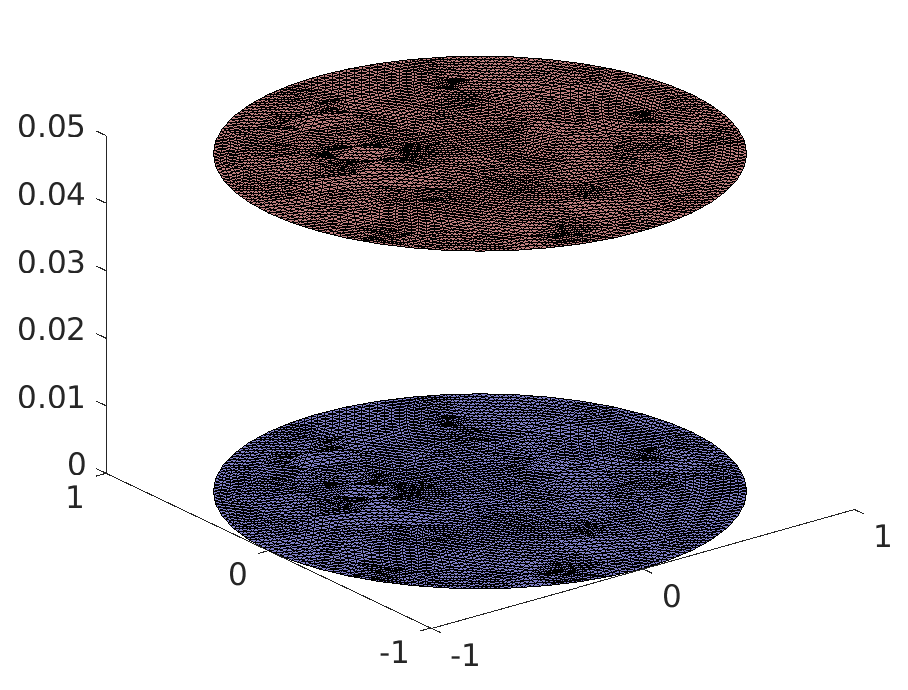
\includegraphics[width=0.48 \textwidth]{fig_article_chap_2/test_case_128/fig_u1u2_hmax0,09_Dt0,001_tt00.eps} 
\quad
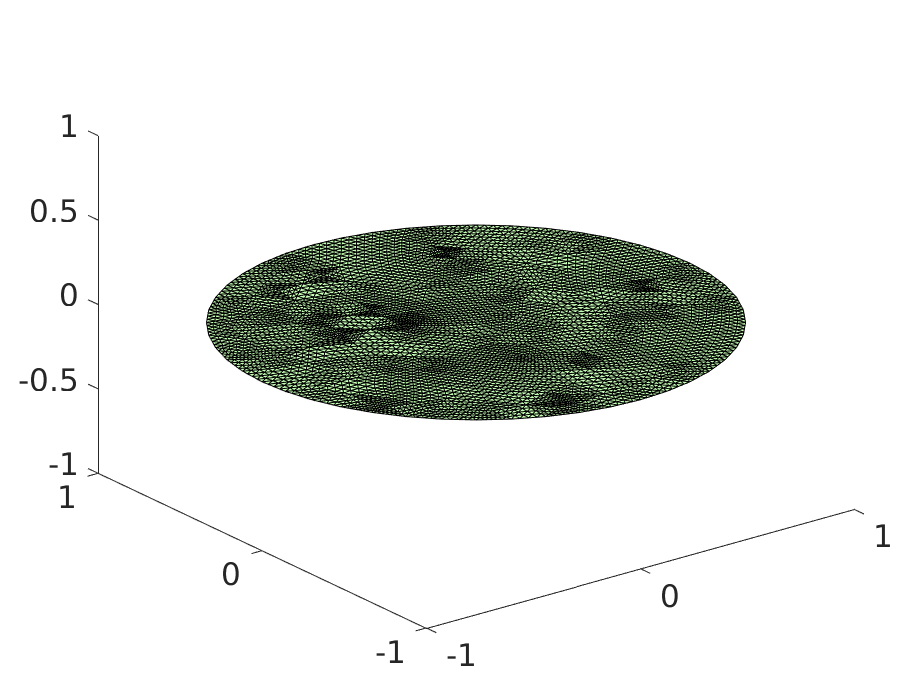
\includegraphics[width=0.48 \textwidth]{fig_article_chap_2/test_case_128/fig_lambda_hmax0,09_Dt0,001_tt02.eps} 
\end{figure}
\onslide<2>
\begin{figure}
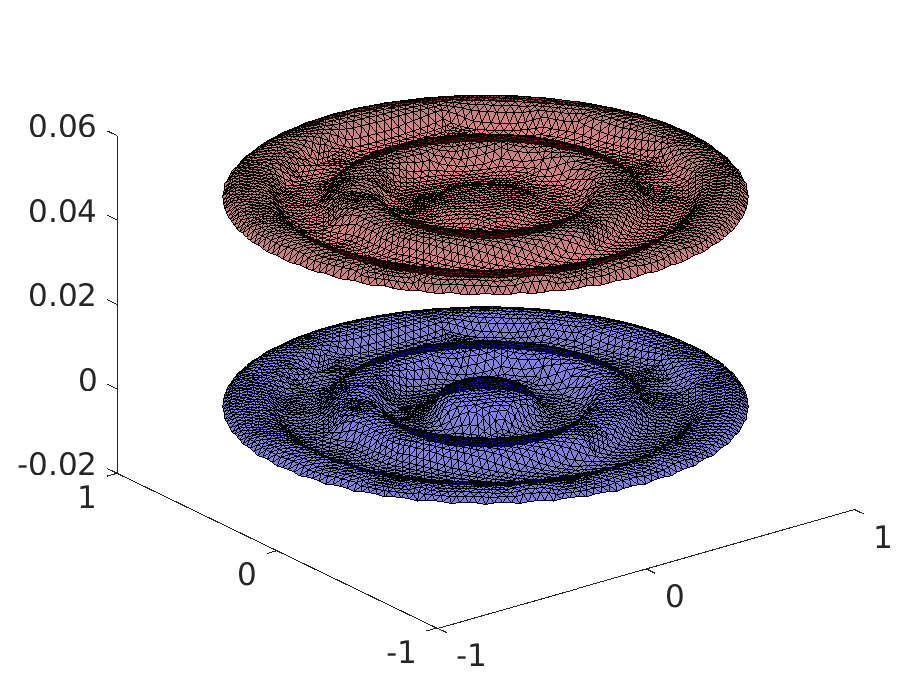
\includegraphics[width=0.48 \textwidth]{fig_article_chap_2/test_case_128/fig_u1u2_hmax0,09_Dt0,001_tt01.eps} 
\quad
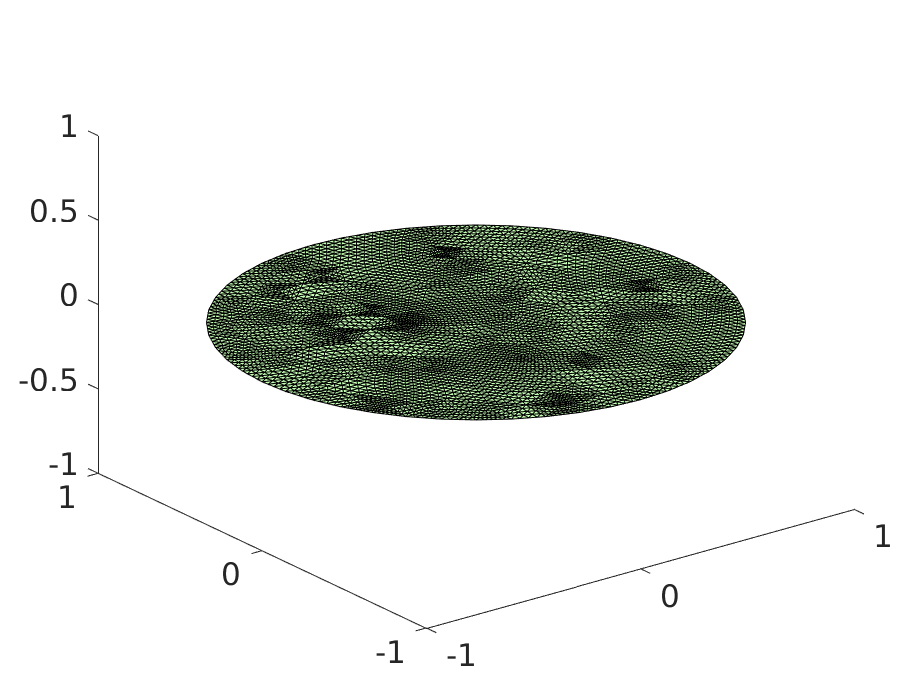
\includegraphics[width=0.48 \textwidth]{fig_article_chap_2/test_case_128/fig_lambda_hmax0,09_Dt0,001_tt02.eps} 
\end{figure}
\onslide<3>
\begin{figure}
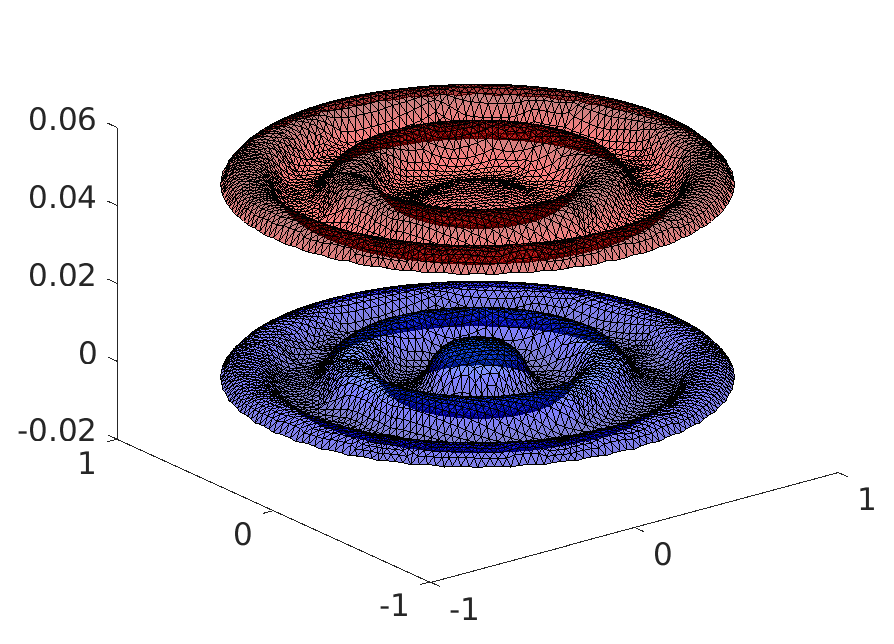
\includegraphics[width=0.48 \textwidth]{fig_article_chap_2/test_case_128/fig_u1u2_hmax0,09_Dt0,001_tt02.eps} 
\quad
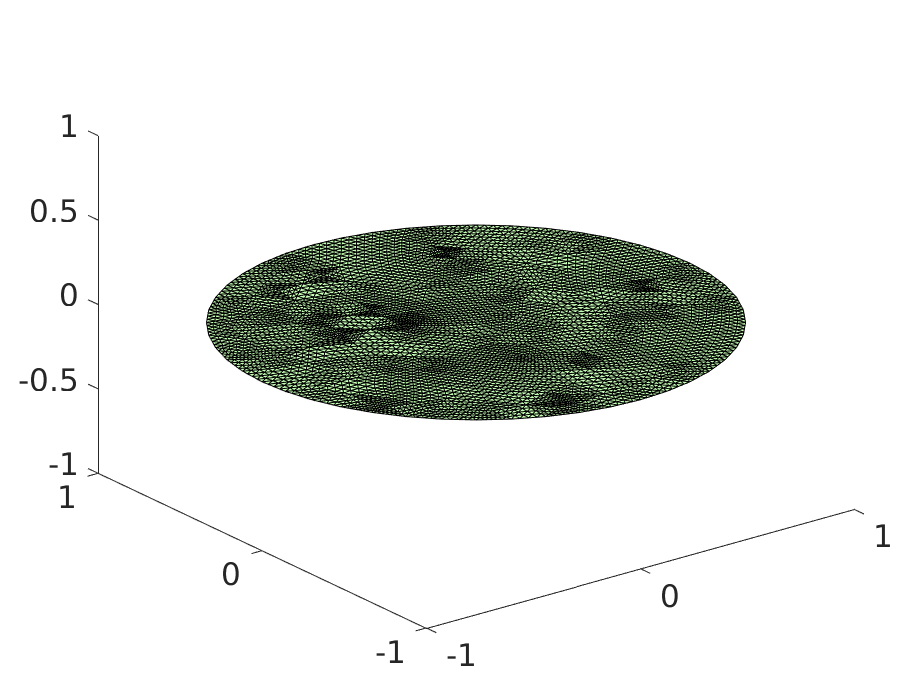
\includegraphics[width=0.48 \textwidth]{fig_article_chap_2/test_case_128/fig_lambda_hmax0,09_Dt0,001_tt02.eps} 
\end{figure}
\onslide<4>
\begin{figure}
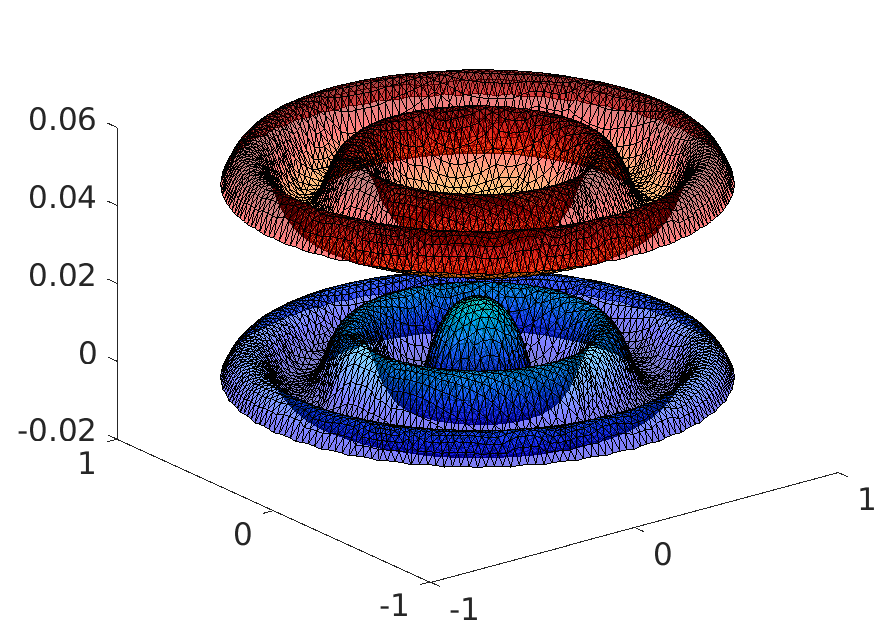
\includegraphics[width=0.48 \textwidth]{fig_article_chap_2/test_case_128/fig_u1u2_hmax0,09_Dt0,001_tt03.eps} 
\quad
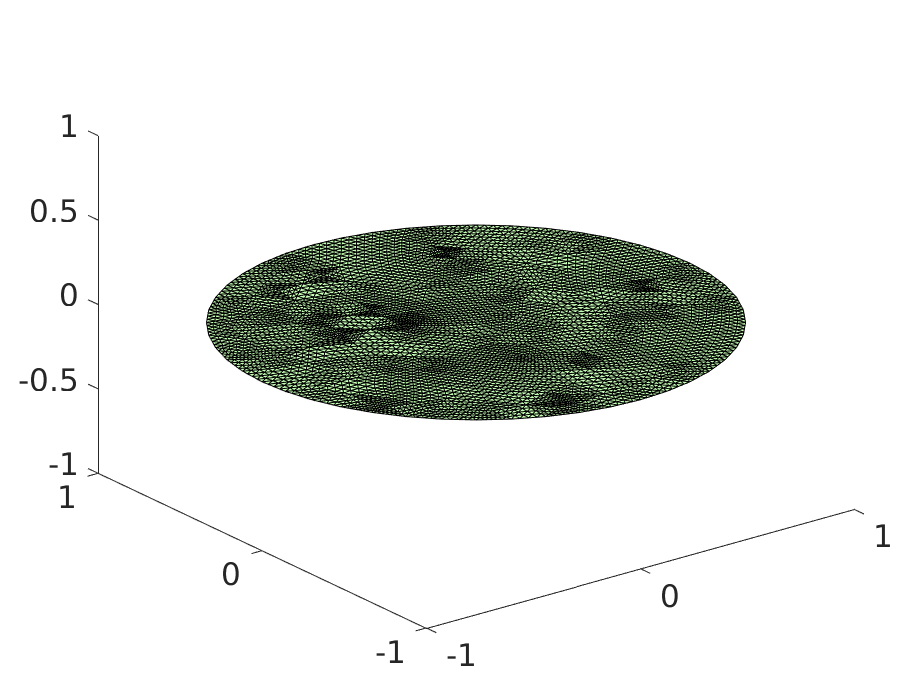
\includegraphics[width=0.48 \textwidth]{fig_article_chap_2/test_case_128/fig_lambda_hmax0,09_Dt0,001_tt02.eps} 
\end{figure}
\onslide<5>
\begin{figure}
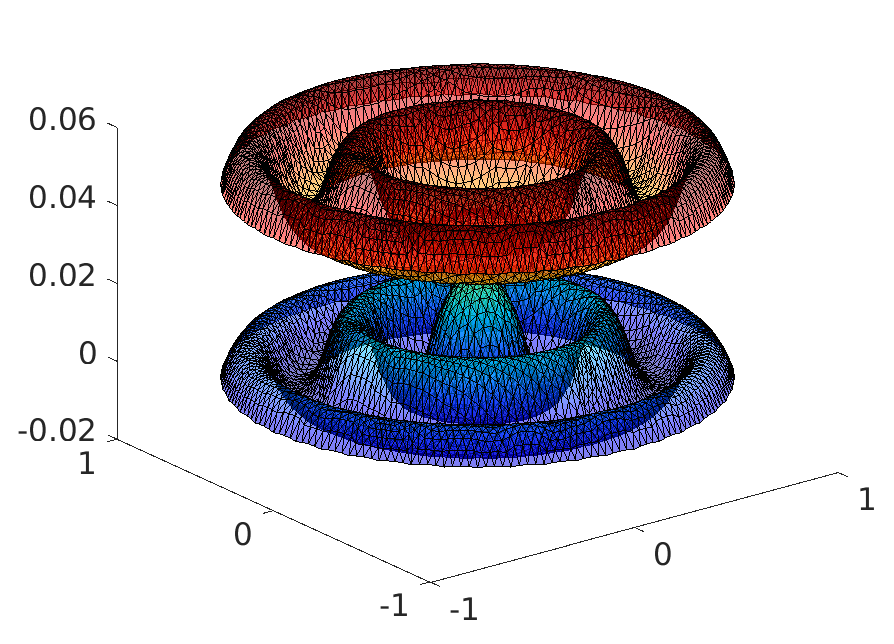
\includegraphics[width=0.48 \textwidth]{fig_article_chap_2/test_case_128/fig_u1u2_hmax0,09_Dt0,001_tt04.eps} 
\quad
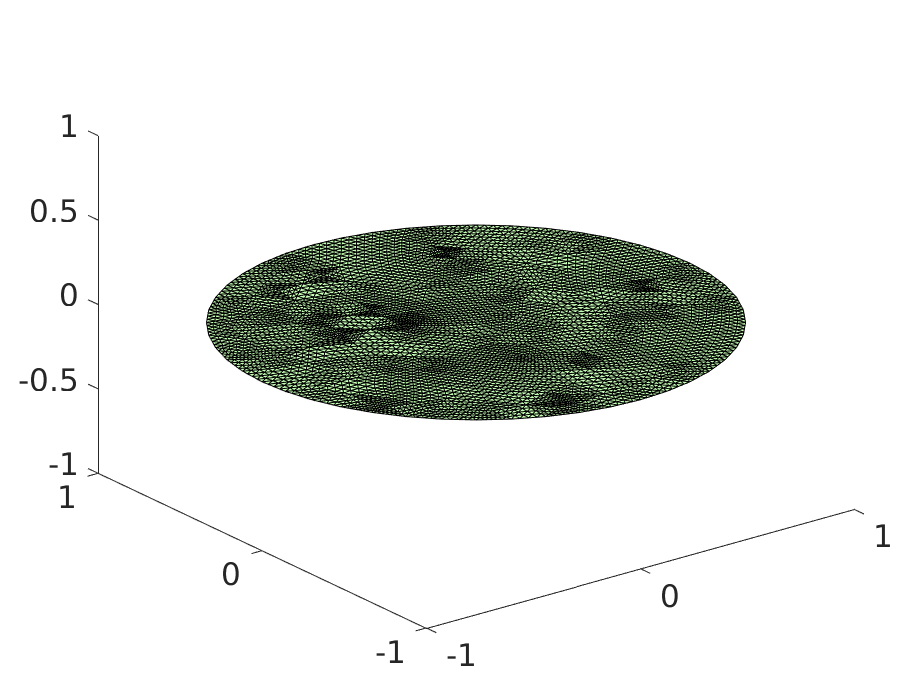
\includegraphics[width=0.48 \textwidth]{fig_article_chap_2/test_case_128/fig_lambda_hmax0,09_Dt0,001_tt02.eps} 
\end{figure}
\onslide<6>
\begin{figure}
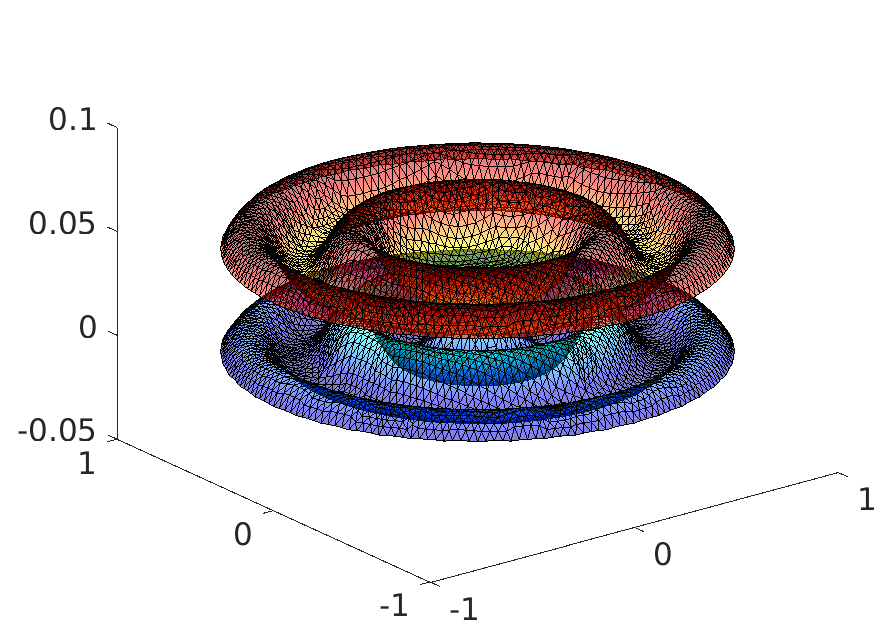
\includegraphics[width=0.48 \textwidth]{fig_article_chap_2/test_case_128/fig_u1u2_hmax0,09_Dt0,001_tt05.eps} 
\quad
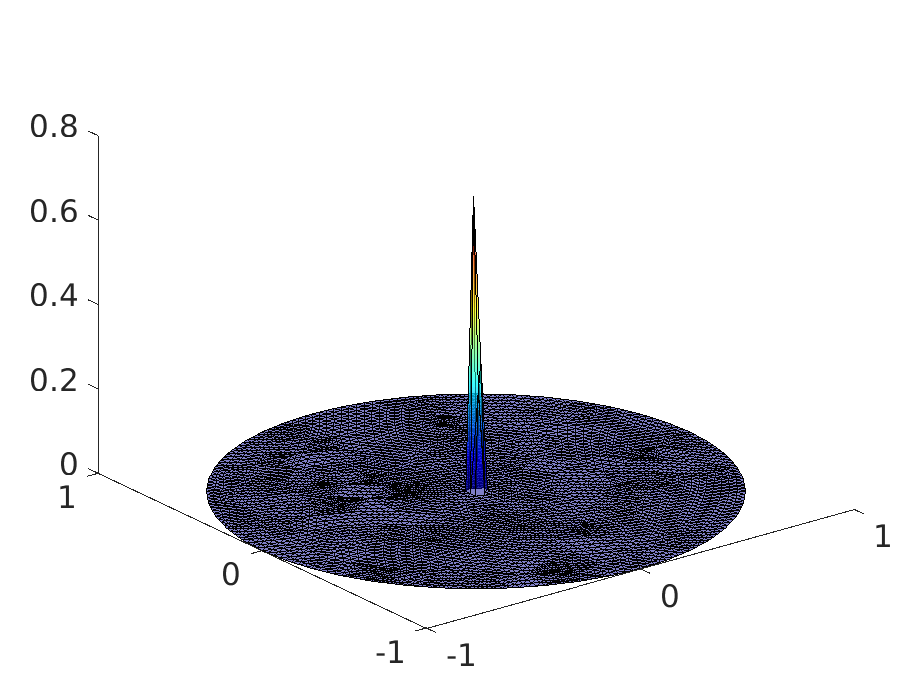
\includegraphics[width=0.48 \textwidth]{fig_article_chap_2/test_case_128/fig_lambda_hmax0,09_Dt0,001_tt05.eps}
\end{figure}
\onslide<7>
\begin{figure}
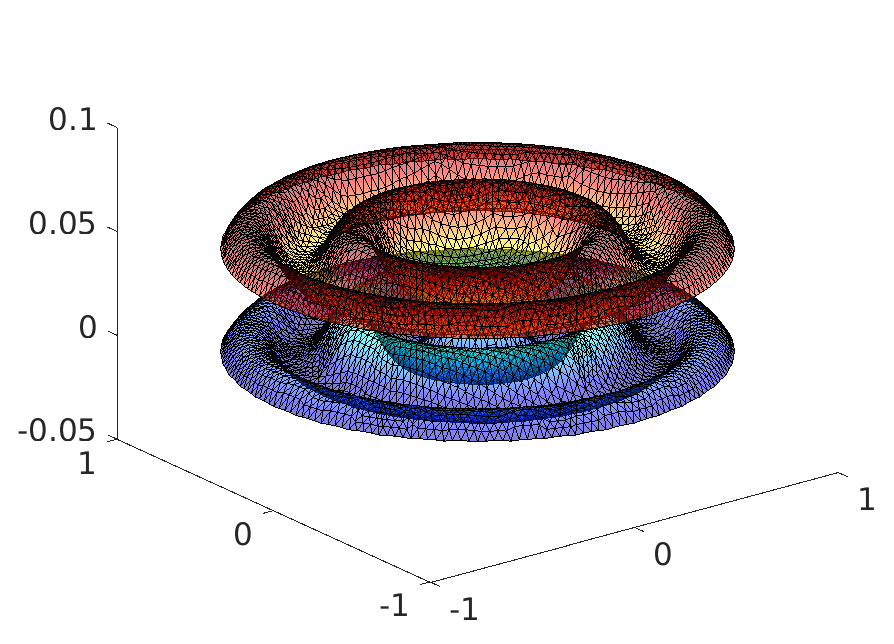
\includegraphics[width=0.48 \textwidth]{fig_article_chap_2/test_case_128/fig_u1u2_hmax0,09_Dt0,001_tt06.eps} 
\quad
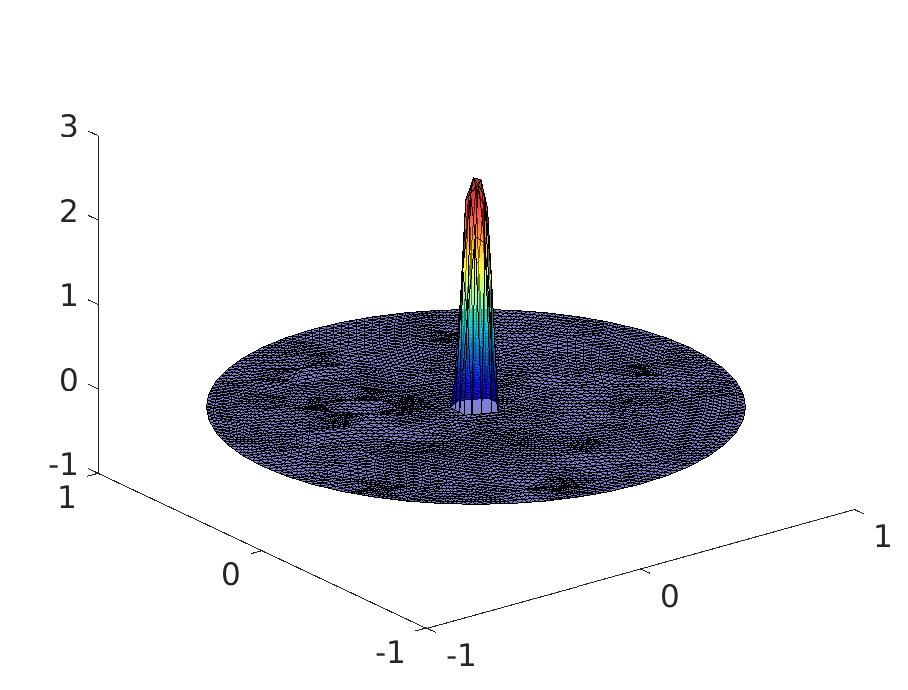
\includegraphics[width=0.48 \textwidth]{fig_article_chap_2/test_case_128/fig_lambda_hmax0,09_Dt0,001_tt06.eps} 
\end{figure}
\onslide<8>
\begin{figure}
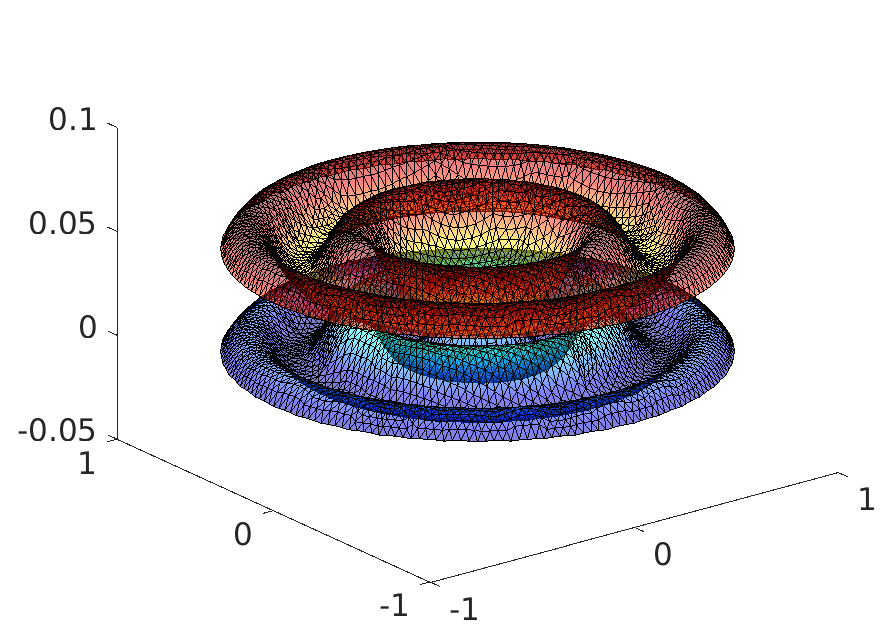
\includegraphics[width=0.48 \textwidth]{fig_article_chap_2/test_case_128/fig_u1u2_hmax0,09_Dt0,001_tt07.eps} 
\quad
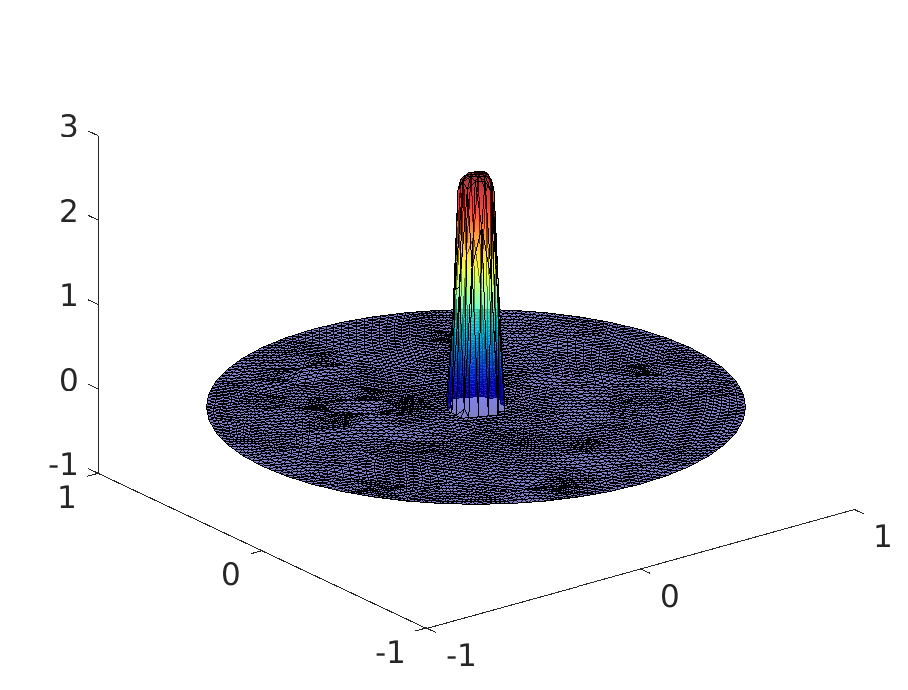
\includegraphics[width=0.48 \textwidth]{fig_article_chap_2/test_case_128/fig_lambda_hmax0,09_Dt0,001_tt07.eps} 
\end{figure}
\onslide<9>
\begin{figure}
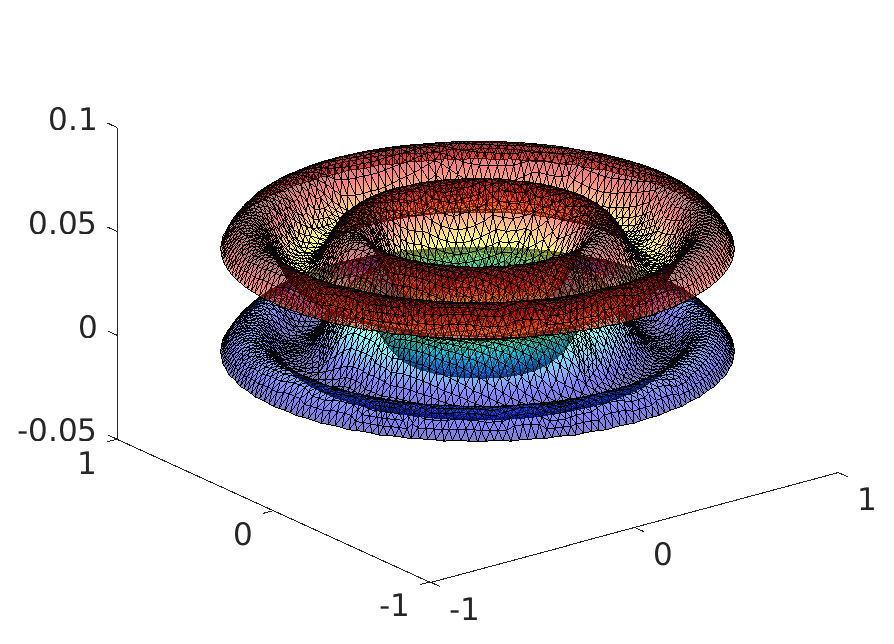
\includegraphics[width=0.48 \textwidth]{fig_article_chap_2/test_case_128/fig_u1u2_hmax0,09_Dt0,001_tt08.eps} 
\quad
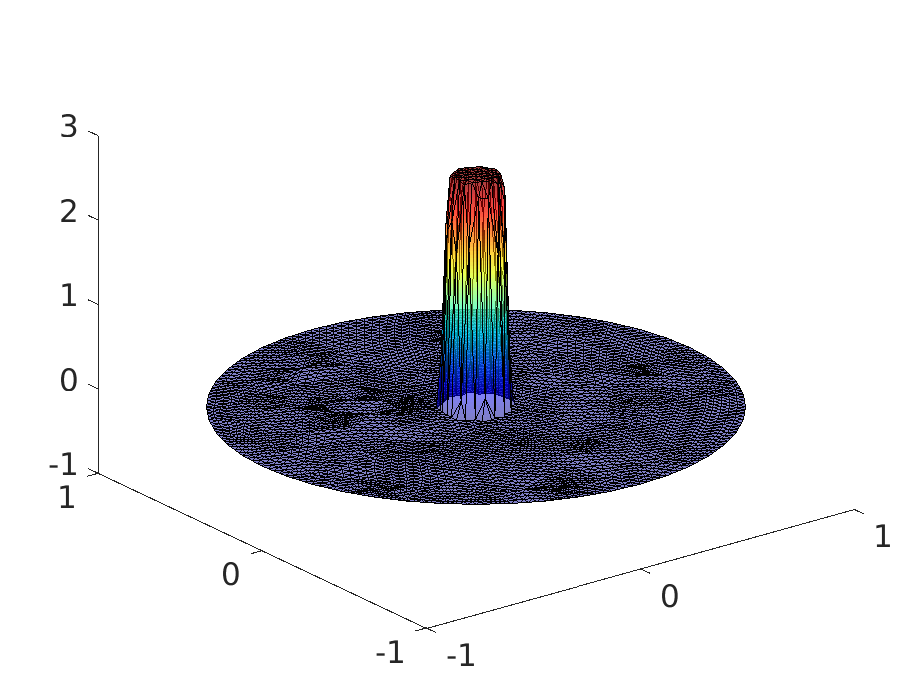
\includegraphics[width=0.48 \textwidth]{fig_article_chap_2/test_case_128/fig_lambda_hmax0,09_Dt0,001_tt08.eps} 
\end{figure}
\onslide<10>
\begin{figure}
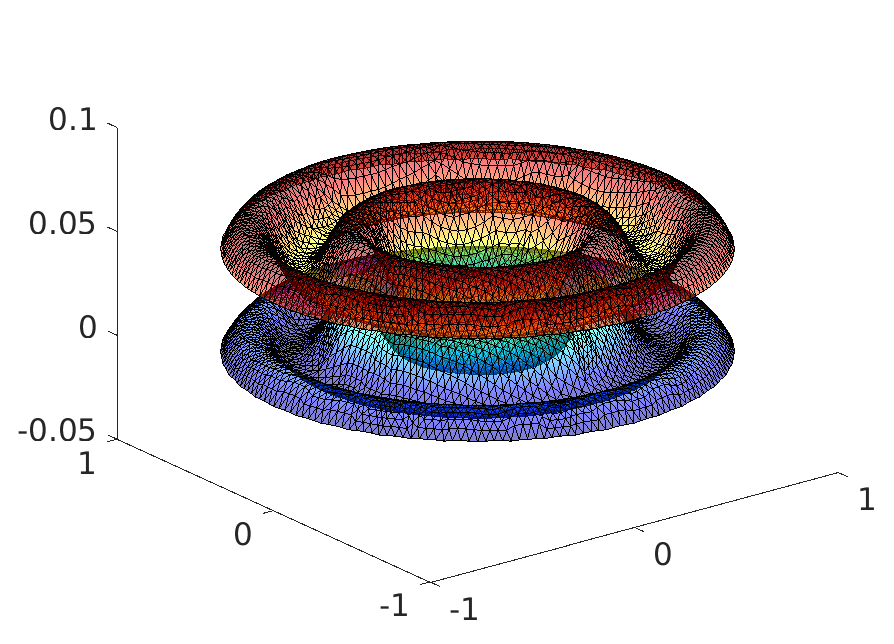
\includegraphics[width=0.48 \textwidth]{fig_article_chap_2/test_case_128/fig_u1u2_hmax0,09_Dt0,001_tt09.eps} 
\quad
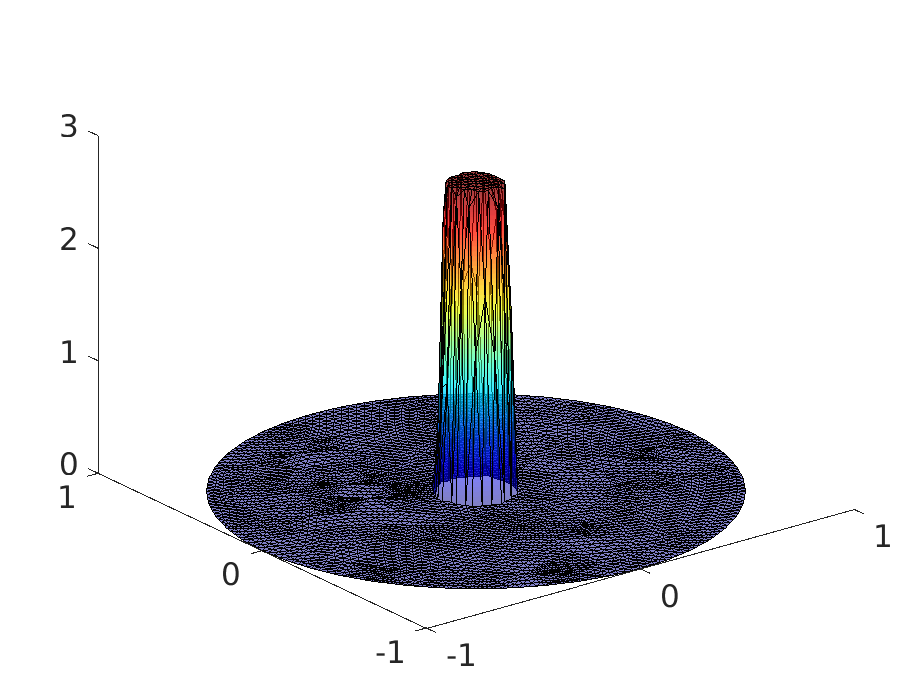
\includegraphics[width=0.48 \textwidth]{fig_article_chap_2/test_case_128/fig_lambda_hmax0,09_Dt0,001_tt09.eps} 
\end{figure}
\onslide<11>
\begin{figure}
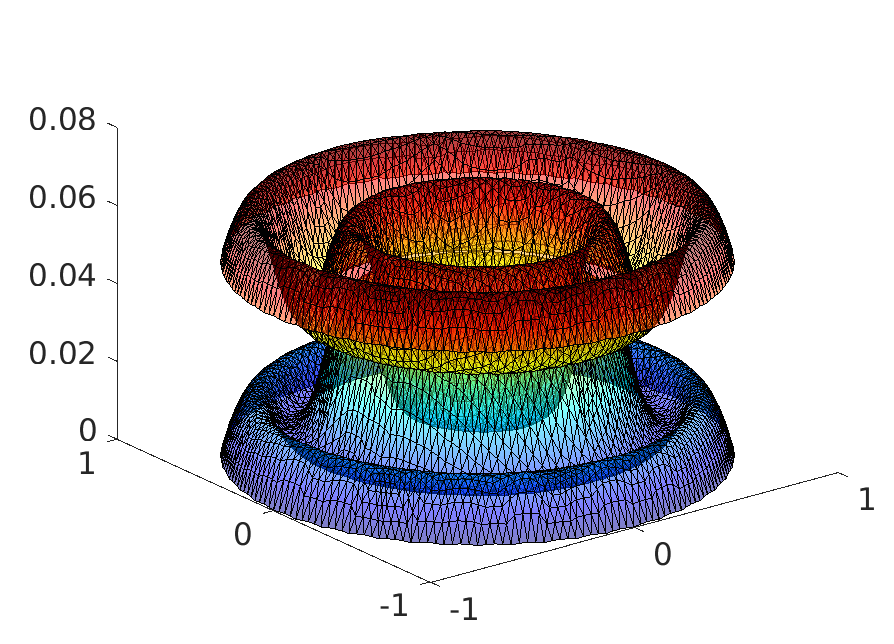
\includegraphics[width=0.48 \textwidth]{fig_article_chap_2/test_case_128/fig_u1u2_hmax0,09_Dt0,001_tt10.eps} 
\quad
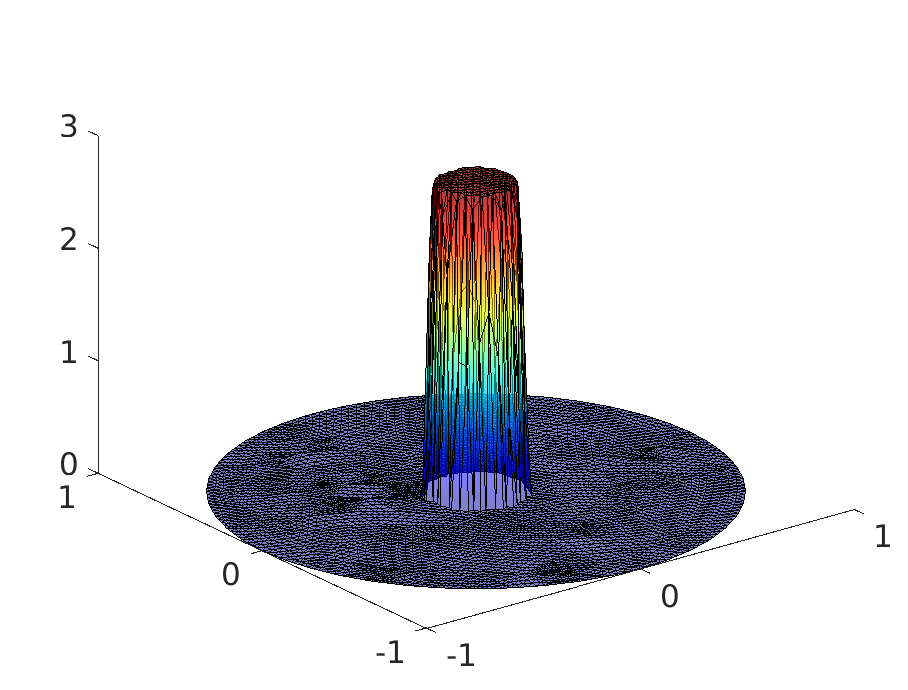
\includegraphics[width=0.48 \textwidth]{fig_article_chap_2/test_case_128/fig_lambda_hmax0,09_Dt0,001_tt10.eps} 
\end{figure}
\onslide<12>
\begin{figure}
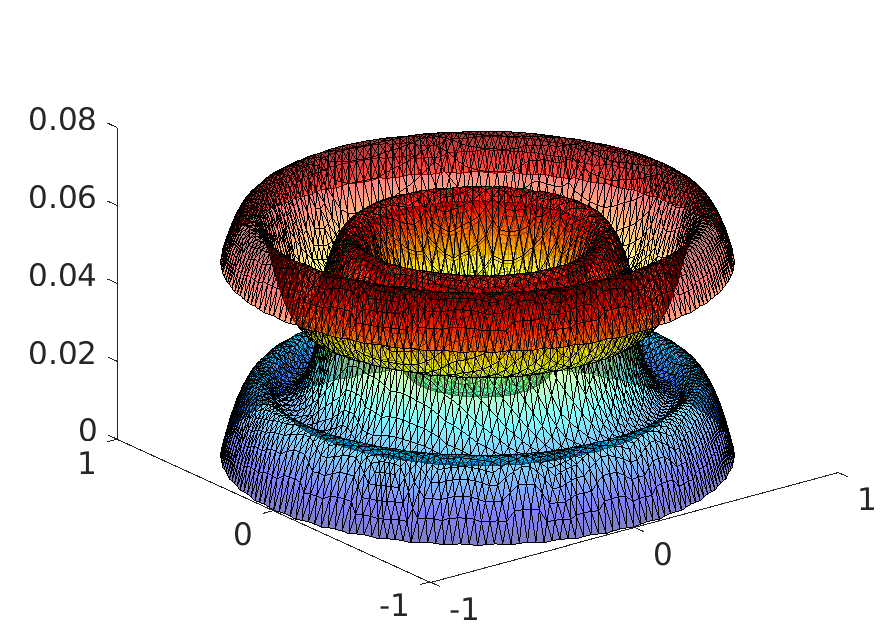
\includegraphics[width=0.48 \textwidth]{fig_article_chap_2/test_case_128/fig_u1u2_hmax0,09_Dt0,001_tt11.eps} 
\quad
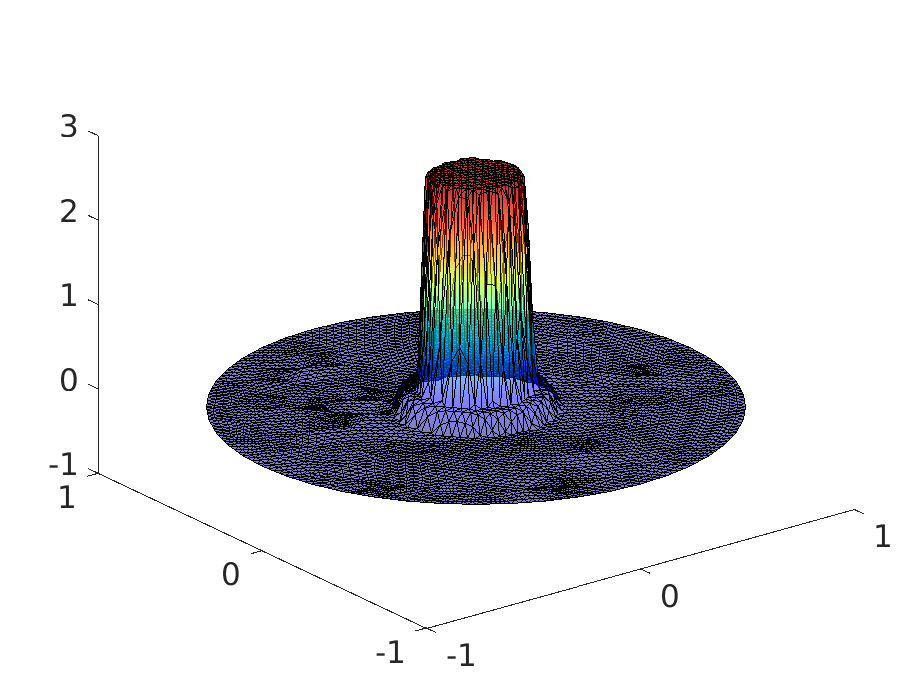
\includegraphics[width=0.48 \textwidth]{fig_article_chap_2/test_case_128/fig_lambda_hmax0,09_Dt0,001_tt11.eps} 
\end{figure}
\onslide<13>
\vspace*{-0.3 cm}
\begin{figure}
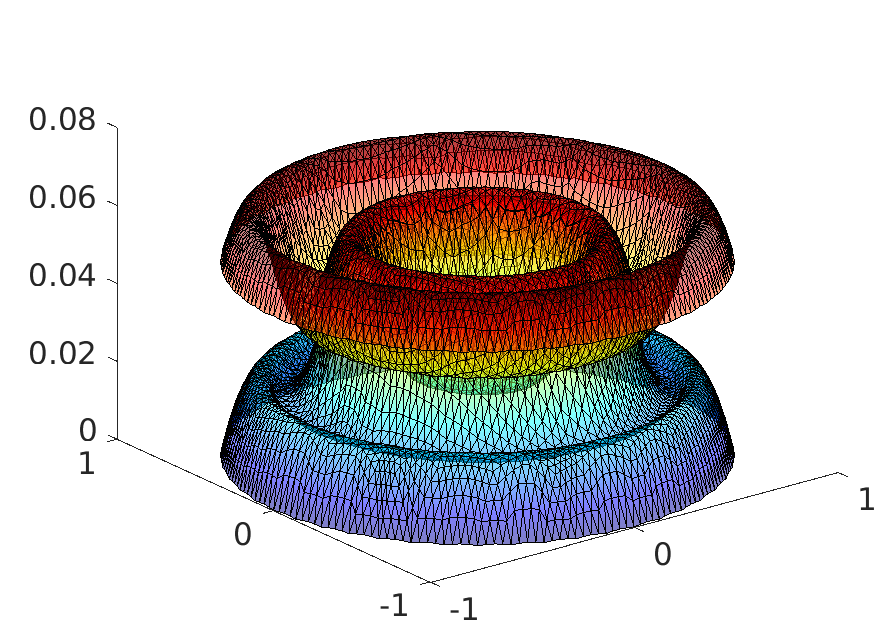
\includegraphics[width=0.48 \textwidth]{fig_article_chap_2/test_case_128/fig_u1u2_hmax0,09_Dt0,001_tt12.eps} 
\quad
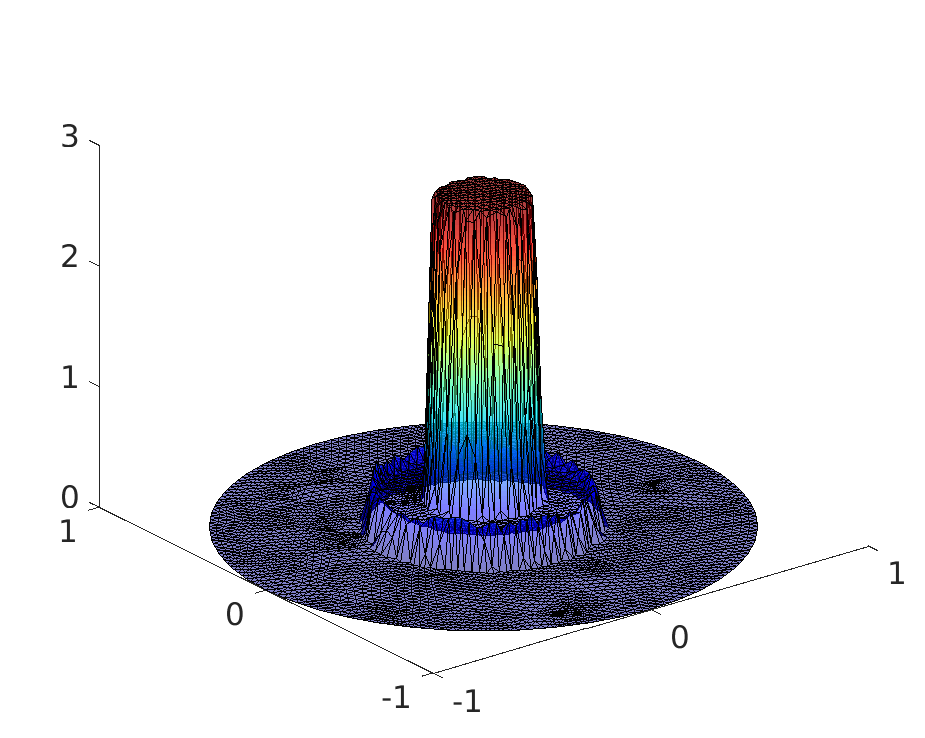
\includegraphics[width=0.48 \textwidth]{fig_article_chap_2/test_case_128/fig_lambda_hmax0,09_Dt0,001_tt12.eps} 
\end{figure}
\onslide<14>
\begin{figure}
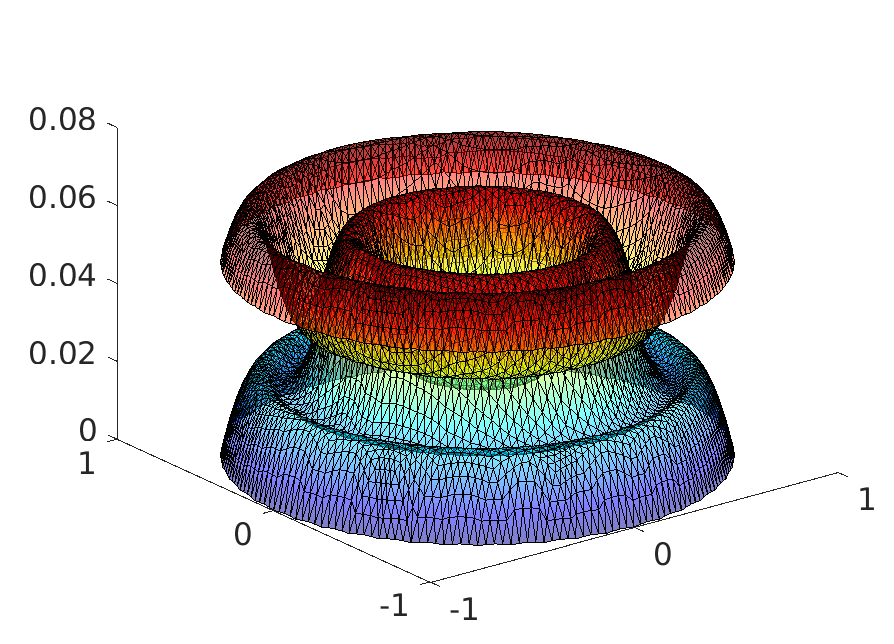
\includegraphics[width=0.48 \textwidth]{fig_article_chap_2/test_case_128/fig_u1u2_hmax0,09_Dt0,001_tt14.eps} 
\quad
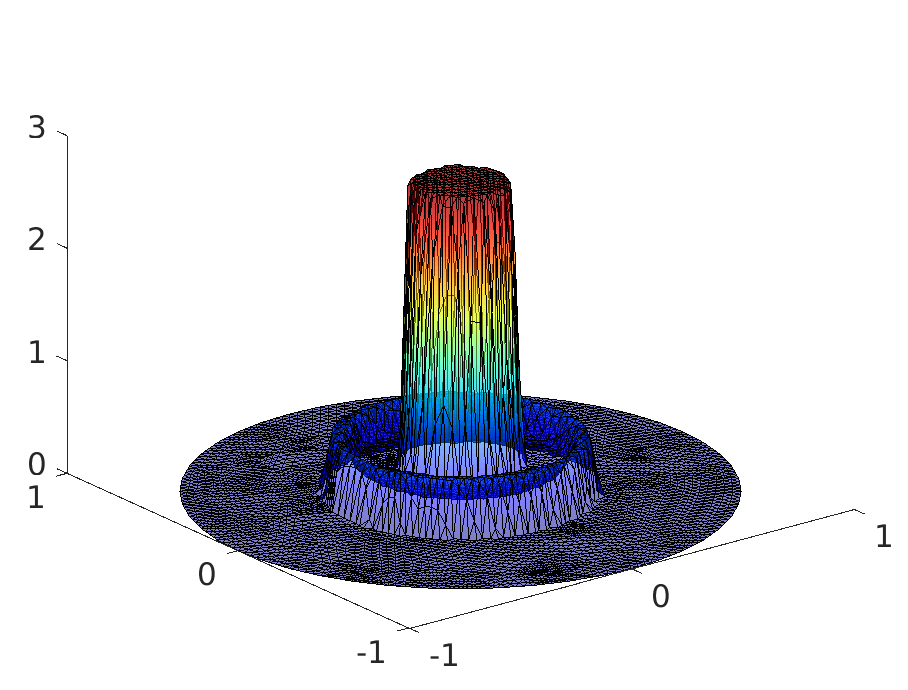
\includegraphics[width=0.48 \textwidth]{fig_article_chap_2/test_case_128/fig_lambda_hmax0,09_Dt0,001_tt14.eps} 
\end{figure}
\end{overprint}
\end{frame}


\begin{frame}
\frametitle{Newton--Fischer--Burmeister adaptivity}
\textcolor{red}{\bm{$\gammalin=\gammaalg=10^{-3}$}}
\begin{figure}
\centering
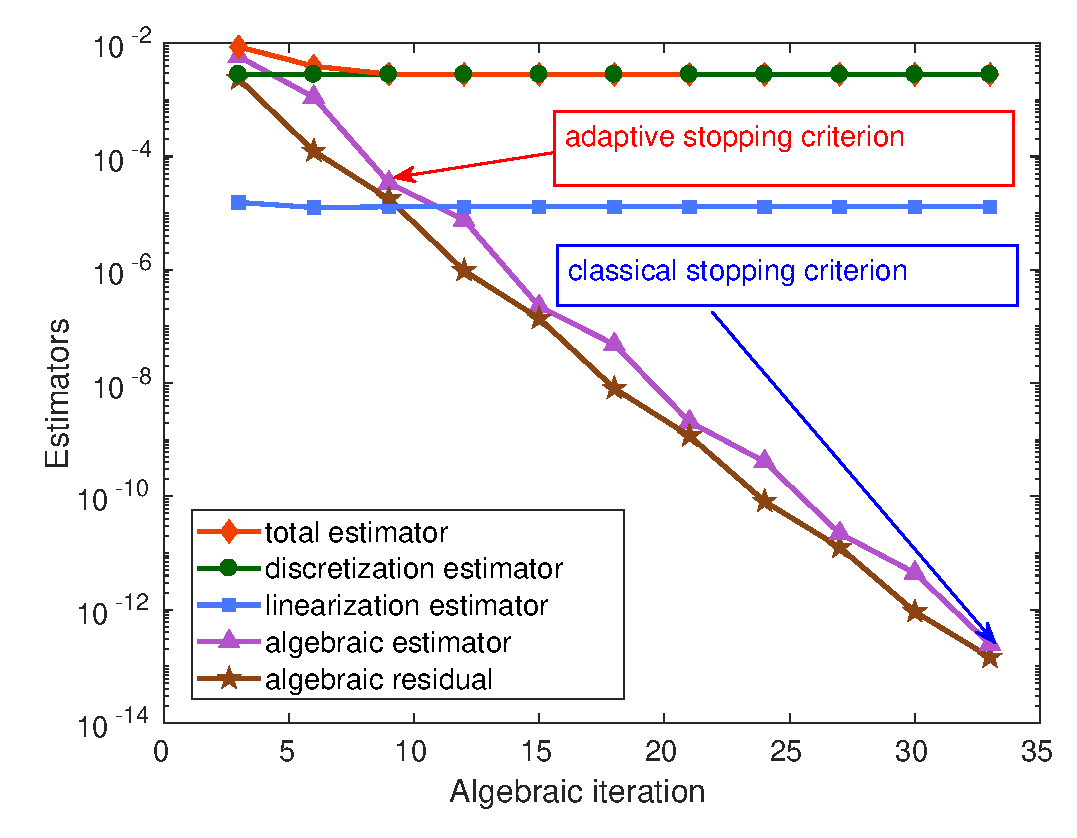
\includegraphics[scale=0.43]{fig_article_chap_2/test_case_1_iter_11_estimator_gmres_1st_newton_iter}
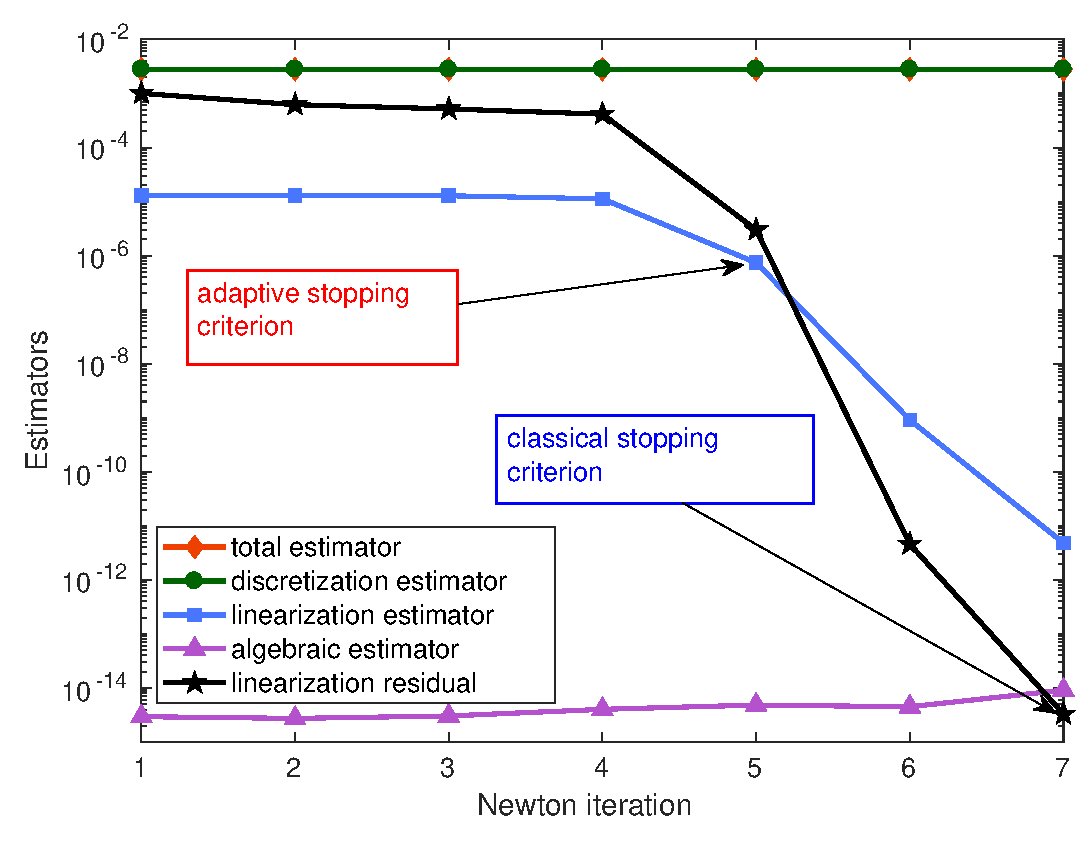
\includegraphics[scale=0.43]{fig_article_chap_2/test_case_1_iter_11_estimator_newton_iter}
\end{figure}
\end{frame}

\begin{frame}
\frametitle{Newton--Fischer--Burmeister performance}
\vspace*{-0.2 cm}
\begin{figure}
\centering
% \includegraphics[width=0.48 \textwidth]{fig_article_chap_2/test_case_128/Number_Newton_FB_iter_time_gamma_10-3} 
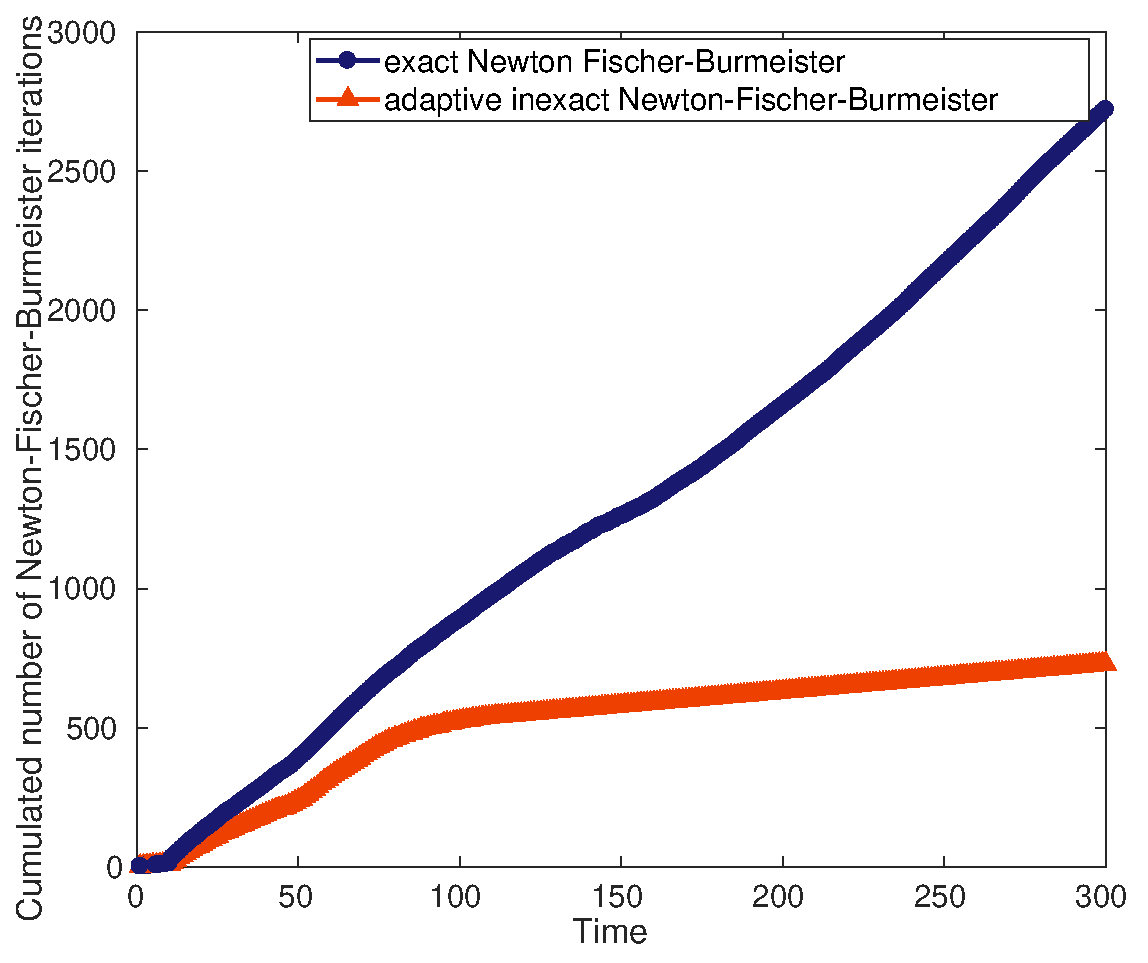
\includegraphics[width=0.45 \textwidth]{fig_article_chap_2/test_case_128/Cumulated_number_Newton_FB_iter_time_gamma_10-3}
\quad
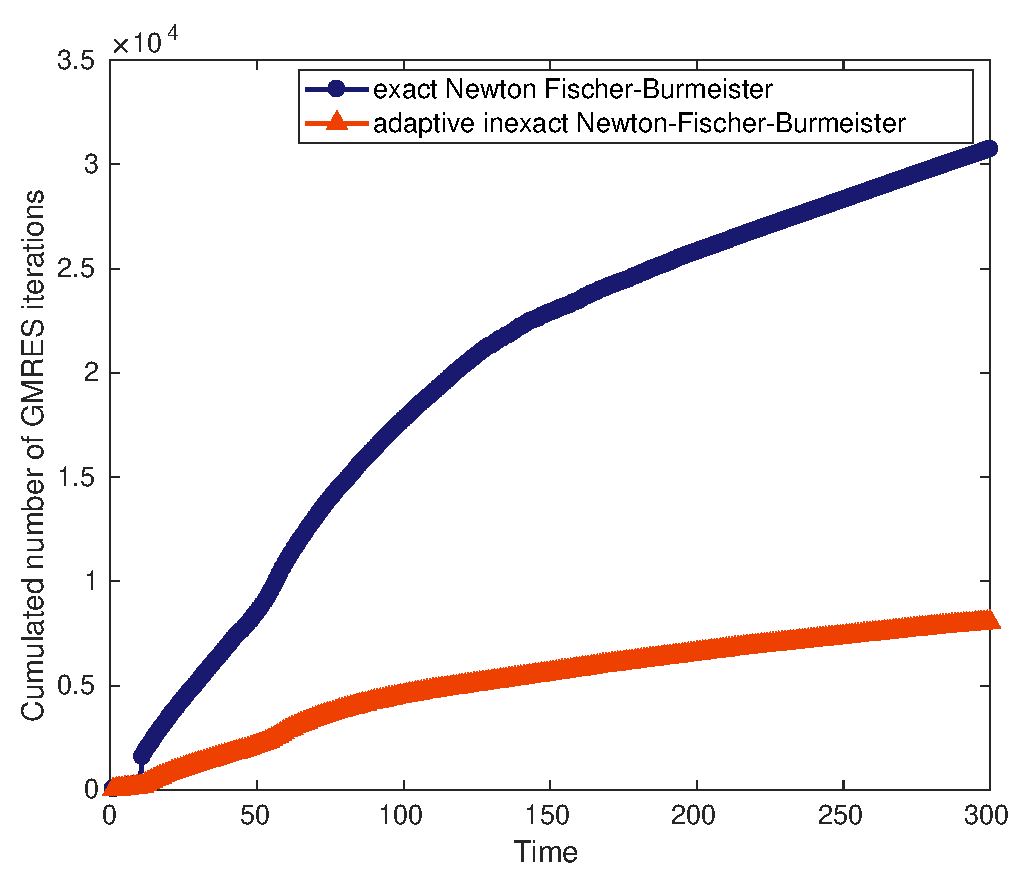
\includegraphics[width=0.45 \textwidth]{fig_article_chap_2/test_case_128/cumulated_number_gmresFB_iter_time_gamma_lin_alg_10-3}
\end{figure}
\vspace*{-0.2 cm}
\begin{thebibliography}{10}
 \scriptsize{
 \bibitem{Dabaghi:Martin:Vohralik:parabolic:2020}
 {\sc J.~Dabaghi, V.~Martin, M.~Vohral\'{i}k}, A posteriori estimates distinguishing the error components and
adaptive stopping criteria for numerical approximations of parabolic variational inequalities.
\em{Computer methods in applied mechanics and engeneering} (2020).
}
 \end{thebibliography}
\end{frame}
%

%% CHAP 3

\begin{frame}
  \frametitle{Two-phase flow with phase appearance and disappearance}
  \textcolor{red}{\textbf{Storage of radioactive wastes in deep geological layers}}
\vspace*{-0.2 cm}
\begin{equation*}
\dps
\left\lbrace\begin{array}{llccc}
\dps \partial_t l_\componentw(\textcolor{cadmiumgreen}{\Sl}) + \nab \cdot {\bm \Phi}_{\mathrm{w}}(\textcolor{cadmiumgreen}{\Sl,\Pl,\chihl}) = Q_{\componentw}, \\
\dps \partial_t l_\componenth(\textcolor{cadmiumgreen}{\Sl,\Pl,\chihl})  + \nab \cdot {\bm \Phi}_{\mathrm{h}}(\textcolor{cadmiumgreen}{\Sl,\Pl,\chihl})=\Qh,\\
\textcolor{electricpurple}{1 - \Sl} \geq 0, \;  \textcolor{carmine}{H\left[\Pl + \Pcp(\Sl) \right] - \beta_{\phasel} \chihl} \geq 0, \; \left[\textcolor{electricpurple}{1 - \Sl} \right] \cdot \left[\textcolor{carmine}{H\left[\Pl + \Pcp(\Sl) \right] - \beta_{\phasel} \chihl}\right]=0  
\end{array}
\right.
\end{equation*}
\vspace{0.1 cm}
\invisible<1>{
\textcolor{midnightblue}{\textbf{Unknowns:}} liquid saturation $\textcolor{cadmiumgreen}{\Sl}$, liquid pressure $\textcolor{cadmiumgreen}{\Pl}$, mole fraction of liquid hydrogen $\textcolor{cadmiumgreen}{\chihl}$ \\
\vspace{0.3 cm}
\invisible<2>{
\textcolor{midnightblue}{\textbf{Linear functions:}} amount of water $l_\componentw$, amount of hydrogen $l_\componenth$\\
\vspace{0.3 cm}
\invisible<3>{
\textcolor{midnightblue}{\textbf{Nonlinear function:}} capillary pressure $\Pcp$ \\
\vspace{0.3 cm}
\invisible<4>{
\textcolor{midnightblue}{\textbf{Nonlinear fluxes:}} water flux $\underbrace{{\bm \Phi}_{\mathrm{w}}}_{\mathrm{Darcy} + \mathrm{Fick}}$, hydrogen flux $\underbrace{{\bm \Phi}_{\mathrm{h}}}_{\mathrm{Darcy} + \mathrm{Fick}}$\\
\vspace{0.3 cm}
\invisible<5>{
\textcolor{midnightblue}{\textbf{Nonlinear complementarity constraints:}} $\Rightarrow$ \textbf{Phase change}\\
\vspace{0.2 cm}
\scriptsize{Ben Gharbia and Jaffré (2014)}

\invisible<6>{
}}}}}}

\end{frame}
%

%
%% DISCRETIZATION FINITE VOLUME
% \begin{frame}
% \frametitle{Discretization by the finite volume method}
% \textcolor{blue}{\textbf{Numerical solution: }}
% \begin{equation*}
% \bUn \egaldef (\bUn_K)_{K\in \Th}, \qquad \bUn_K \egaldef  (\SKn,\PKn,\chiKn) \quad \textcolor{cadmiumgreen}{\textbf{one value per cell and time step}} 
% \label{eq:finite:volume:approx}
% \end{equation*}
% \textcolor{cadmiumgreen}{\textbf{Time discretization:}}
% \\
%  \begin{figure}[htbp]
% \vspace{-0.6 cm}
%  \centering
%  \begin{picture}(200,60)(0,0)
%  \thicklines
%  \put(0,15){\line(200,0){200}}
%  %\put(0,10){\red{\line(0,10){10}}}
%  \put(0,0){\makebox(0,0){\small \red{$t_0 = 0$}}}
%  \put(0,15){\black{\circle*{6}}}
%  \put(25,10){\red{\line(0,10){10}}}
%  \put(25,0){\makebox(0,0){\small \red{$t_1$}}}
%  %\put(25,15){\blue{\circle*{6}}}
%  \put(12.5,30){\makebox(0,0){\small  \blue{$I_1$}}}
%  \put(50,10){\red{\line(0,10){10}}}
%  \put(50,0){\makebox(0,0){\small \red{$t_2$}}}
%  %\put(75,15){\blue{\circle*{6}}}
%  \put(37.5,30){\makebox(0,0){\small  \blue{$I_2$}}}
%  \put(75,30){\makebox(0,0){\small \blue{$\cdots$}}}
%  \put(75,0){\makebox(0,0){\small \red{$\cdots$}}}
%  \put(112.5,30){\makebox(0,0){\small \blue{$I_{n}$}}}
%  %\put(215,15){\blue{\circle*{6}}}
%  \put(100,10){\red{\line(0,10){10}}}
%  \put(100,0){\makebox(0,0){\red{\small $t_{n-1}$}}}
%  \put(125,10){\red{\line(0,10){10}}}
%  \put(125,0){\makebox(0,0){\red{\small $t_{n}$}}}
%  \put(150,30){\makebox(0,0){\small \blue{$\cdots$}}}
%  \put(150,0){\makebox(0,0){\small \red{$\cdots$}}}
%  \put(175,0){\makebox(0,0){\small \red{$t_{\Nt - 1}$}}}
%  \put(175,10){\red{\line(0,10){10}}}
%  %\put(355,15){\blue{\circle*{6}}}
%  \put(187.5,30){\makebox(0,0){\small \blue{$I_{\Nt}$}}}
%  \put(200,0){\makebox(0,0){\small \red{$t_{\Nt} = t_{\mathrm{F}}$}}}
%  %\put(240,10){\red{\line(0,10){10}}}
%  \put(200,15){\black{\circle*{6}}}
%  \end{picture}
% \qquad \qquad
% 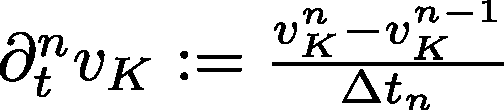
\includegraphics[scale = 0.5]{fig_article_chap_2/approx_time_derivative.pdf}
%  \end{figure}
% \begin{minipage}[c]{0.3 \textwidth}
% \textcolor{cadmiumgreen}{\textbf{Space discretization:}} $\Th$ a superadmissible family of conforming simplicial meshes of $\Omega$. \textcolor{blue}{Number of cells : $\Nsp$}
% \begin{equation*}
% \dps 
% \left(\nab v \cdot \bn_{K,\sigma},1\right)_{\sigma} := \dps |\sigma| \frac{v_L - v_K}{d_{KL}} \hspace{0.2 cm} \sigma = \overline{K} \cap \overline{L},
% \end{equation*}
% \end{minipage}
% \hfill
% \begin{minipage}[c]{0.5 \textwidth}
% \begin{figure}
% 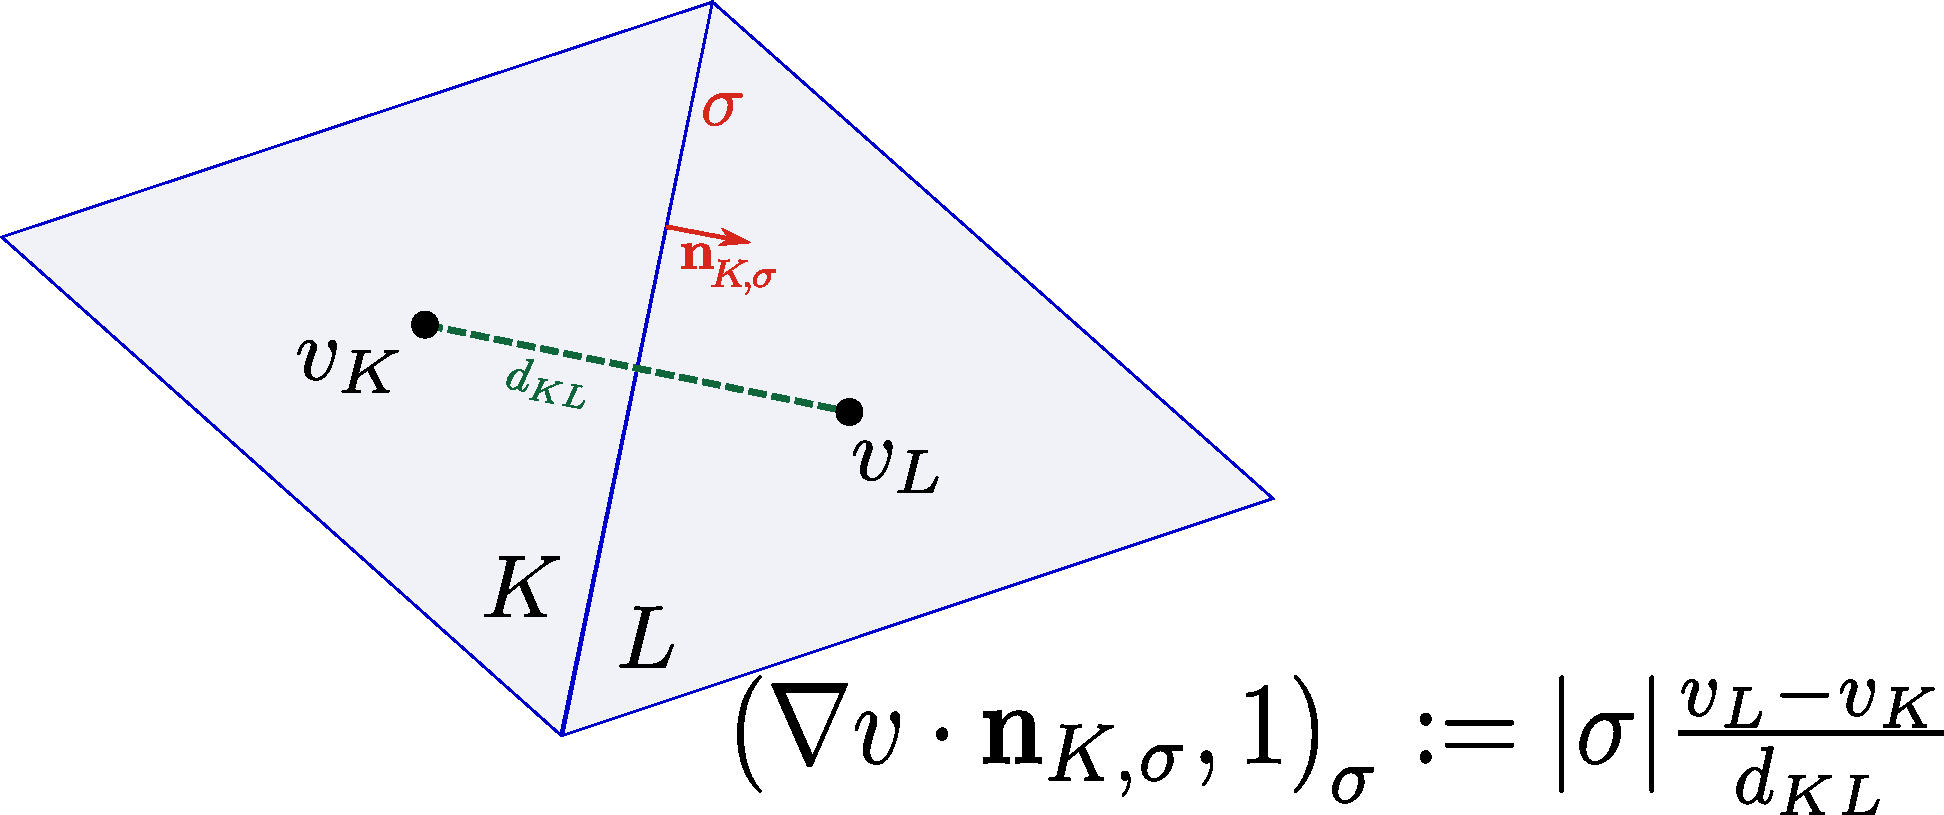
\includegraphics[width = 0.7 \textwidth]{fig_article_chap_3/gradient_discretization.pdf}
% \end{figure}
% \end{minipage}
% \end{frame}

\begin{frame}
\frametitle{Discretization by the finite volume method}
\textcolor{cadmiumgreen}{\textbf{Numerical solution: }}
\begin{equation*}
 \bUn \egaldef (\bUn_K)_{K\in \Th}, \qquad \bUn_K \egaldef  (\SKn,\PKn,\chiKn) \quad \textcolor{cadmiumgreen}{\textbf{one value per cell and time step}} 
\end{equation*}
\textcolor{blue}{\textbf{Discretization of the water equation}}
\begin{equation*}
S_{\mathrm{w},K}^n(\bU^n) \egaldef |K| \partial_t^n \lwK  + \sum_{\sigma \in \EK} {F}_{\componentw,K,\sigma}(\bU^{n})- |K|\QwKn = 0,
\end{equation*}
% \begin{equation*}
% {F}_{\componentw,K,\sigma}(\bUn) \egaldef \rhowl (\mobilityliq)_{\sigma}^{n} (\psil)_{\sigma}^{n} - (\jhl)_{\sigma}^{n} \quad \sigma \in \EKint \quad \overline{\sigma} = \overline{K} \cap \overline{L}.
% \end{equation*}
\invisible<1>{
\textcolor{blue}{\textbf{Discretization of the hydrogen equation}}
\begin{equation*} 
S_{\mathrm{h},K}^{n}(\bU^n)\egaldef |K| \partial_t^n \lhK + \sum_{\sigma \in \EK} {F}_{\componenth,K,\sigma}(\bUn) - |K| \QhKn = 0,
\end{equation*}
% \begin{equation*}
%  {F}_{\componenth,K,\sigma}(\bUn) \egaldef \betal \chisigman (\mobilityliq)_{\sigma}^{n} (\psil)_{\sigma}^{n} + (\psig)_{\sigma}^{n} (\mobilitygas)_{\sigma}^{n} (\rhog)_{\sigma}^{n} + (\jhl)_{\sigma}^{n} , \quad \sigma \in \EKint \quad \overline{\sigma} = \overline{K} \cap \overline{L}.
% \end{equation*}
\invisible<2>{
At each time step $t^n$, we obtain the nonlinear system of algebraic equations
\begin{equation*}
S_{c,K}^n(\bU^n)=0 \quad \forall K \in \Th \ \ \forall \componentc \in \left\{\componentw,\componenth\right\}
\end{equation*}
\invisible<3>{
}}}
\end{frame}
%
\begin{frame}
\frametitle{Discrete complementarity problem and semismoothness}
\textcolor{red}{\textbf{Discretization of the nonlinear complementarity constraints}}
\begin{equation*}
\textcolor{electricpurple}{\mathcal{K}(\bU_K^n)} \egaldef \textcolor{electricpurple}{1-\SKn} \quad \textcolor{carmine} {\mathcal{G}(\bU_K^n)} \egaldef  \textcolor{carmine}{H(\PKn\hspace{-0.05 cm}+\hspace{-0.05 cm}\Pcp(\SKn))-\betal \chiKn}
\end{equation*}
\pause
The discretization reads
\begin{equation*}
\begin{split}
&S_{c,K}^n(\bU^n)=0 \quad \forall K \in \Th \quad \forall \componentc \in \left\{\componentw,\componenth \right\}\\
& \textcolor{electricpurple}{\mathcal{K}(\bU_K^n)} \geq 0, \quad   \textcolor{carmine} {\mathcal{G}(\bU_K^n)} \geq 0, \quad \textcolor{electricpurple}{\mathcal{K}(\bU_K^n)} \cdot \textcolor{carmine} {\mathcal{G}(\bU_K^n)}=0 \quad \forall K \in \Th
\end{split}
\end{equation*}
\pause
\begin{itemize}
\item
\textcolor{cadmiumgreen}{\textbf{We reformulate the complementarity constraints with C-functions}}
\item
\textcolor{cadmiumgreen}{\textbf{We employ inexact semismooth linearization}}
\item
\textcolor{cadmiumgreen}{\textbf{Can we estimate the error?}}
\item
\textcolor{cadmiumgreen}{\textbf{Can we distinguish the error components?}}
\end{itemize}
\end{frame} 
%
%%
\begin{frame}
\frametitle{Weak solution}
\begin{equation*}
X \egaldef L^2((0,\tF);H^1(\Omega)), \ Y  \egaldef H^1((0,\tF);L^2(\Omega)), 
%\ \widehat{Y} \egaldef H^1((0,\tF);L^{\infty}(\Omega)),\\
 \  Z \egaldef L_{+}^2((0,\tF);L^{\infty}(\Omega)) 
% \\ & \left\| \varphi \right\|_{X_n} \egaldef \int_{\In} \sum_{K \in \Th} \left(\varepsilon h_K^{-2} \left\|\varphi\right\|_K^2 + \left\|\nab \varphi\right\|_K^2\right) (t) \mathrm{dt}
\end{equation*}
\\
\vspace{0.5 cm}
\textcolor{blue}{\textbf{Assumption: There exists a unique weak solution satisfying}}
\begin{itemize}
\item
% $\Sl \in \widehat{Y}$, \ 
$\textcolor{electricpurple}{1-\Sl} \in Z$, \ $\lc \in Y$, \ $\Pl \in X$, \ $\chihl \in X$, \ $\Phic \in L^2((0,\tF); \HdivOmeg)$
\item 
$\dps \int_{0}^{\tF} \left(\partial_t \lc, \varphi \right)_{\Omega}(t)\,\mathrm{dt}-\hspace{-0.1 cm}\int_{0}^{\tF} \left(\Phic, \nab \varphi \right)_{\Omega}(t)\,\mathrm{dt} = \hspace{-0.1 cm} \int_{0}^{\tF} \left(\Qc, \varphi \right)_{\Omega}(t)\,\mathrm{dt} \quad \forall \varphi \in X$
\item 
$\dps \int_{0}^{\tF} \left(\lambda - \left(\textcolor{electricpurple}{1 - \Sl}\right), \textcolor{carmine}{H[\Pl+\Pcp(\Sl)]-\betal \chihl}  \right)_{\Omega}(t)\,\mathrm{dt} \geq 0 \quad \forall \lambda \in Z$
\item
the initial condition  holds
\end{itemize}
\end{frame}
% %

\begin{frame}
\frametitle{Error measure}
\vspace{-0.3 cm}
\begin{enumerate}
\item<1> 
\textcolor{cadmiumgreen}{\textbf{Dual norm of the residual for the components}}
 \begin{equation*}
\left\|\mathcal{R}_{\componentc}(\Shtaunki,\Phtaunki,\chihtaunki) \right\|_{\Xn'} \egaldef \sup_{\substack{\varphi \in \Xn \\ \left\|\varphi\right\|_{\Xn} = 1}}  \int_{\In} 
 \left(\Qc - \partial_t \lchtaunki , \varphi\right)_{\Omega}(t) + \left(\Phichtaunki,\nab \varphi \right)_{\Omega}(t)\,\mathrm{dt} 
 \end{equation*}
\pause
\item<2>
\textcolor{cadmiumgreen}{\textbf{Residual for the constraints}}
\begin{equation*}
  \mathcal{R}_{\mathrm{e}}(\Shtaunki,\Phtaunki,\chihtaunki) \egaldef \int_{\In}\left(\textcolor{electricpurple}{1 - \Shtaunki}, \textcolor{carmine}{H \left[\Phtaunki + \Pcp(\Shtaunki)\right] - \betal \chihtaunki} \right)_{\Omega}(t)\,\mathrm{dt}
\end{equation*}
\pause
\item<3>
\textcolor{cadmiumgreen}{\textbf{Error measure for the nonconformity of the pressure}} $\mathcal{N}_{p}(\Phtaunki)$
\pause
\item<4>
\textcolor{cadmiumgreen}{\textbf{Error measure for nonconformity of the molar fraction}} $\mathcal{N}_{\chi}(\chihtaunki)$
\end{enumerate}
\vspace{0.3 cm}
\begin{equation*}
\mathcal{N}^{n,\kk,\ii}  \egaldef \left\{\sum_{\componentc \in\mathcal{C}} \left\|\mathcal{R}_{\componentc}(\Shtaunki,\Phtaunki,\chihtaunki) \right\|_{X_n'}^2 \right\}^{\frac{1}{2}} + \left\{\sum_{\phasep \in \mathcal{P}}\mathcal{N}_{\phasep}^2 + \mathcal{N}_{\chi}^2\right\}^{\frac{1}{2}} + \mathcal{R}_{\mathrm{e}}(\Shtaunki,\Phtaunki,\chihtaunki)
\end{equation*}
\end{frame}
\begin{frame}
  \frametitle{Post-processing}
The discrete liquid pressure and discrete molar fraction \textcolor{midnightblue}{\textbf{are piecewise constant}} 
\\
\begin{equation*}
\left(\PKnki\right)_{K \in \Th} \in \textcolor{cadmiumgreen}{\PzeroTh} \quad \left(\chiKnki\right)_{K \in \Th} \in \textcolor{cadmiumgreen}{\PzeroTh}
\end{equation*}
Piecewise polynomial reconstruction:
\begin{equation*}
\Phnki \in \textcolor{cadmiumgreen}{\PtwoTh}, \quad \chihnki \in \textcolor{cadmiumgreen}{\PtwoTh}
\end{equation*}
\vspace{-0.1 cm}
Conforming reconstruction:
\begin{equation*}
\tildePhnki \in \textcolor{cadmiumgreen}{\PtwoTh} \ \textcolor{red}{\bm \cap} \ H^1(\Omega), \quad \tildechihnki \in \textcolor{cadmiumgreen}{\PtwoTh} \ \textcolor{red}{\bm \cap} \ H^1(\Omega).
\end{equation*}
\vspace{-0.8 cm}
\begin{figure}
\centering
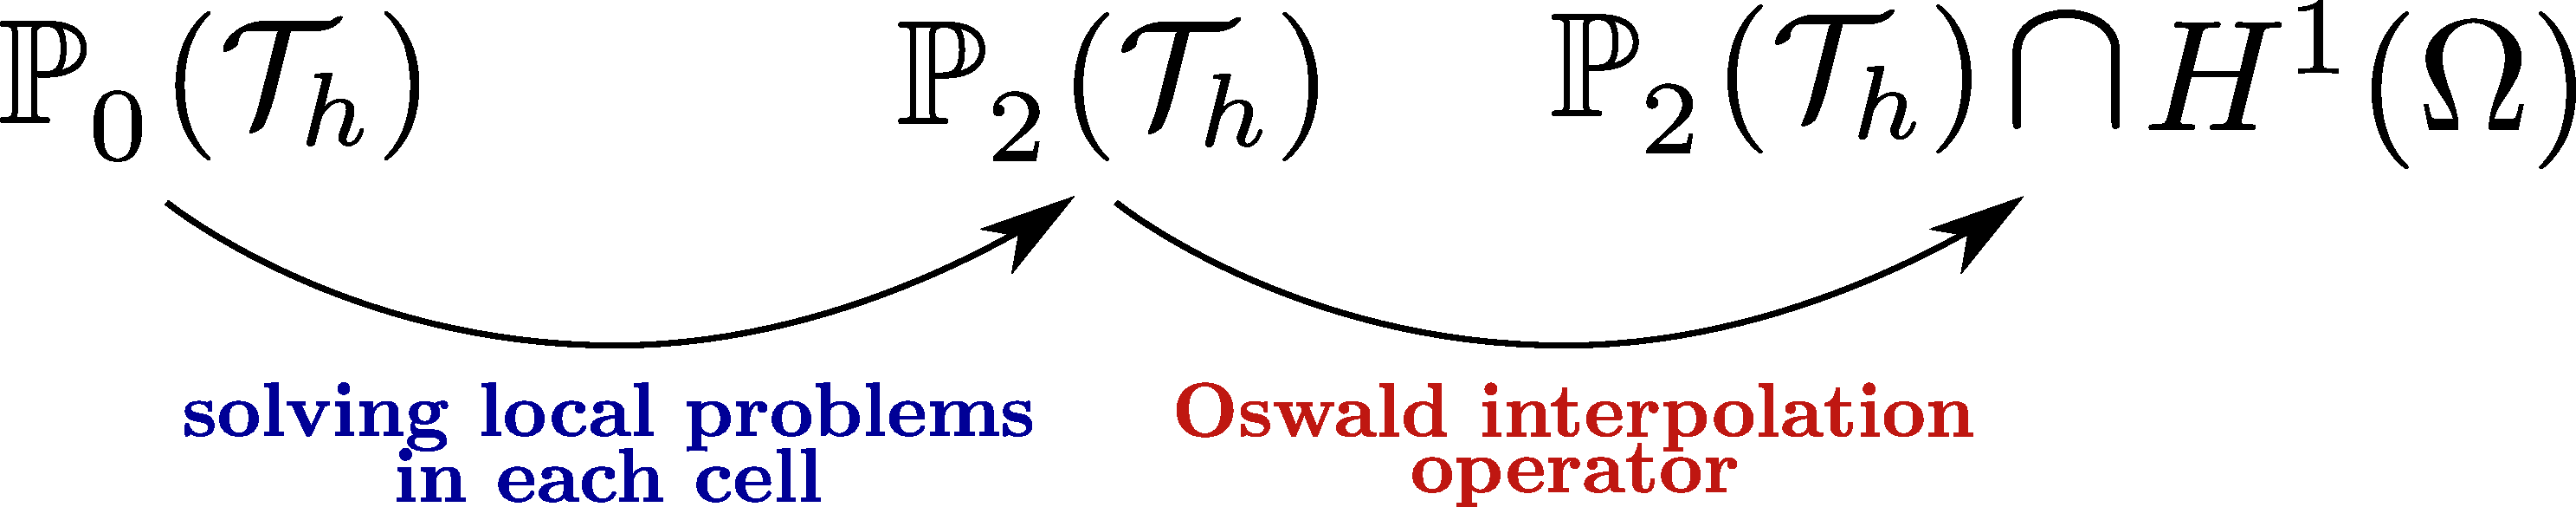
\includegraphics[width = 0.6 \textwidth]{fig_article_chap_3/image_oswald2}
\end{figure}
\end{frame}
%%%
\begin{frame}
\frametitle{A posteriori error estimate distinguishing the error components}

\begin{theorem}
\begin{equation*}
\mathcal{N}^{n,\kk,\ii} \leq \etadiscnki + \etalinnki + \etaalgnki
\end{equation*}
\end{theorem}
\textcolor{red}{Construction of the estimators:} 
\begin{itemize}
\item Equilibrated component flux reconstruction in $\HdivOmeg$
\item Potential reconstruction in $H^1(\Omega)$ 
\end{itemize}
\end{frame}
%

% 
\begin{frame}
\frametitle{Numerical experiments}
$\Omega$:  one-dimensional core with length $L = 200 m$. 
\\
\vspace{0.2 cm}
\textbf{Semismooth solver:} Newton-min
\\
\vspace{0.2 cm}
\textbf{Iterative algebraic solver:} GMRES.
\\
\vspace{0.2 cm}
\textbf{Time step:} $\Delta t = 5000$ years, 
\\
\vspace{0.2 cm}
\textbf{Number of cells:} $\Nsp = 1000$, \\
\vspace{0.2 cm}
\textbf{Final simulation time:} $\tF = 5 \times 10^{5}$ years.
\\
\vspace{0.2 cm}
\begin{figure}
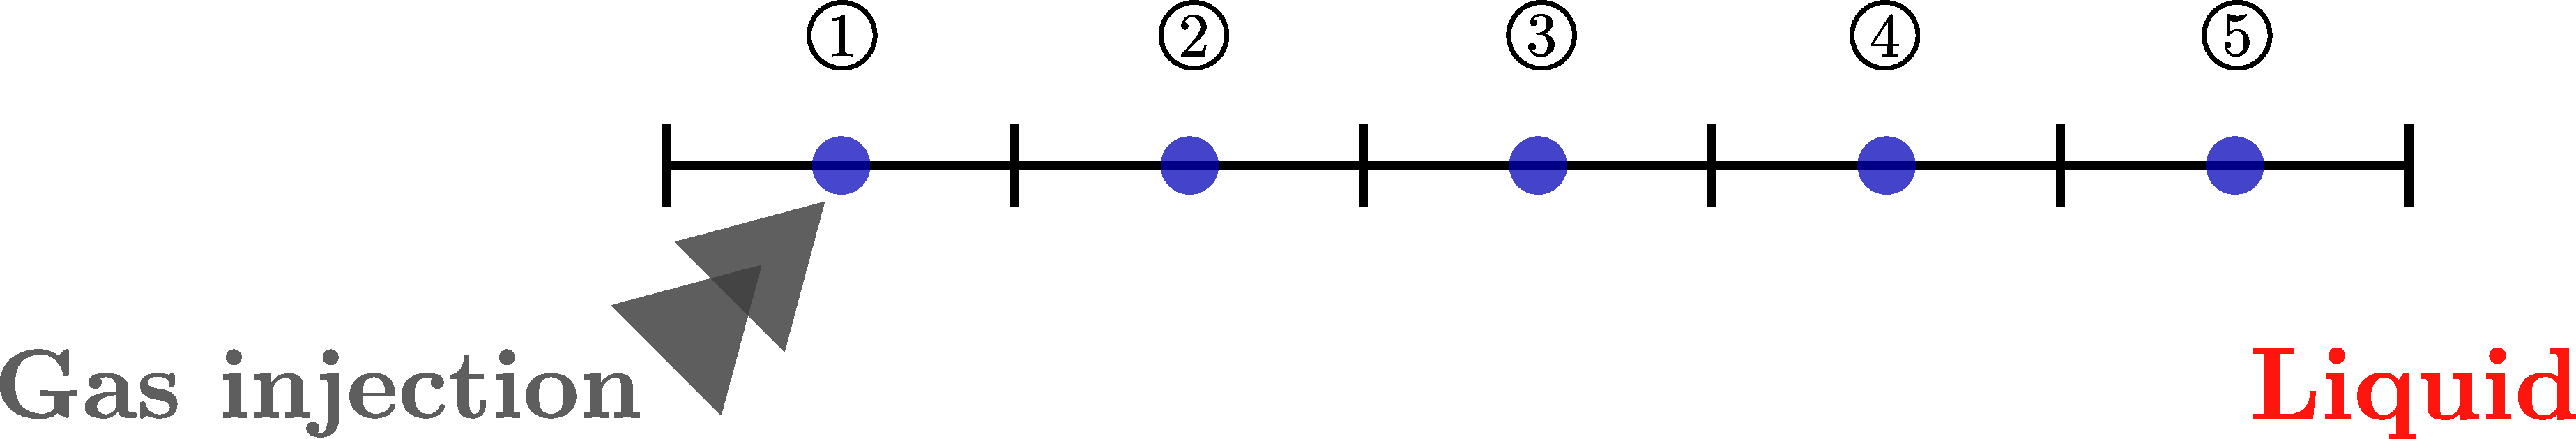
\includegraphics[width= 1 \textwidth]{fig_article_chap_3/num_exp_finite_vol}
\end{figure}

\end{frame}
% 

\begin{frame}
\frametitle{Phase transition estimator}

  \begin{overprint}
    \onslide<1> \scriptsize{\textcolor{red}{\textbf{\bm{$t=2500$} years}}} 
\begin{figure}
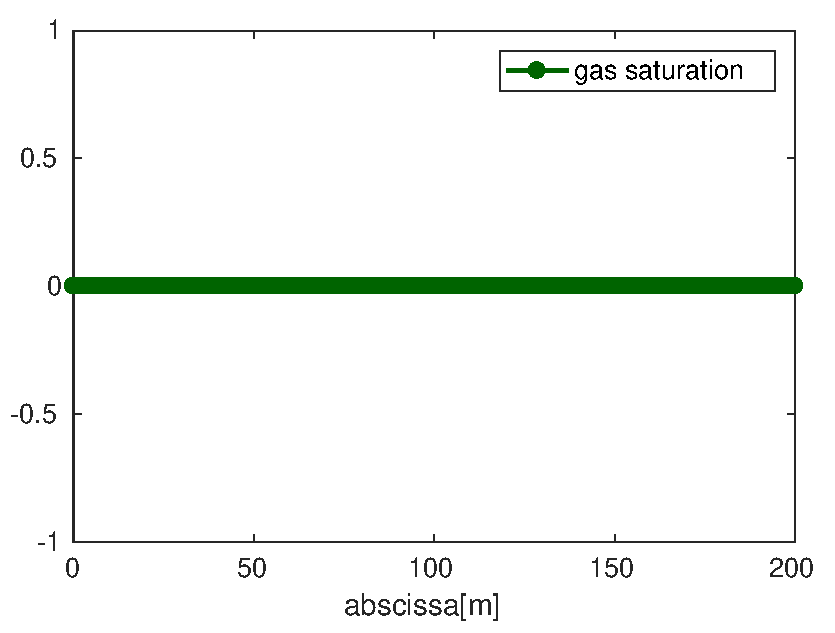
\includegraphics[width=0.47\textwidth]{fig_article_chap_3/satur_gas_init_time2}
\quad
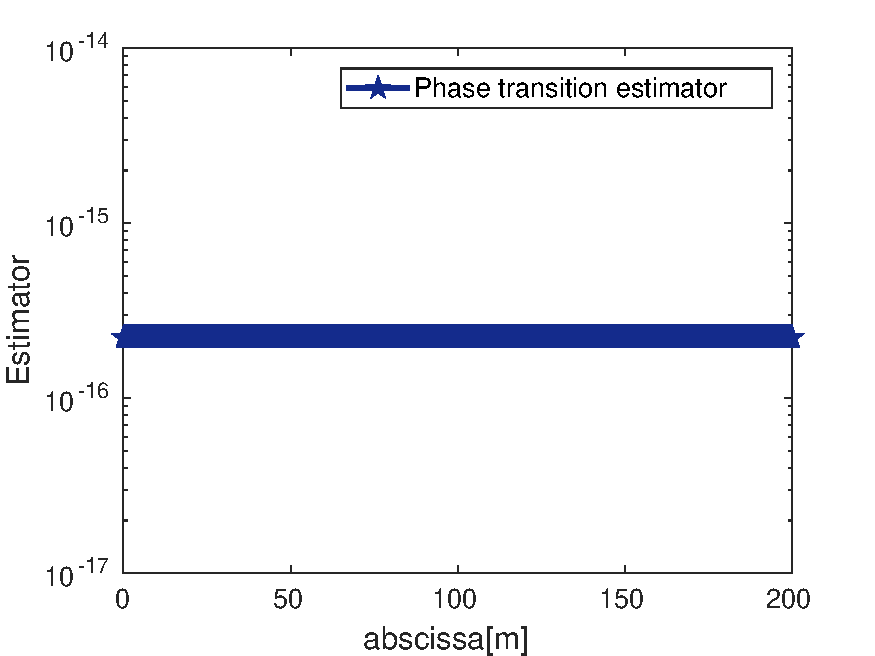
\includegraphics[width=0.47\textwidth]{fig_article_chap_3/MODIF_phase_transition_estimator_appearance_gas_nt=inittime_cv} 
    \end{figure}
\onslide<2>
\scriptsize{\textcolor{red}{ \textbf{\bm{$t = 1.25 \times 10^4$} years}}}
\begin{figure}
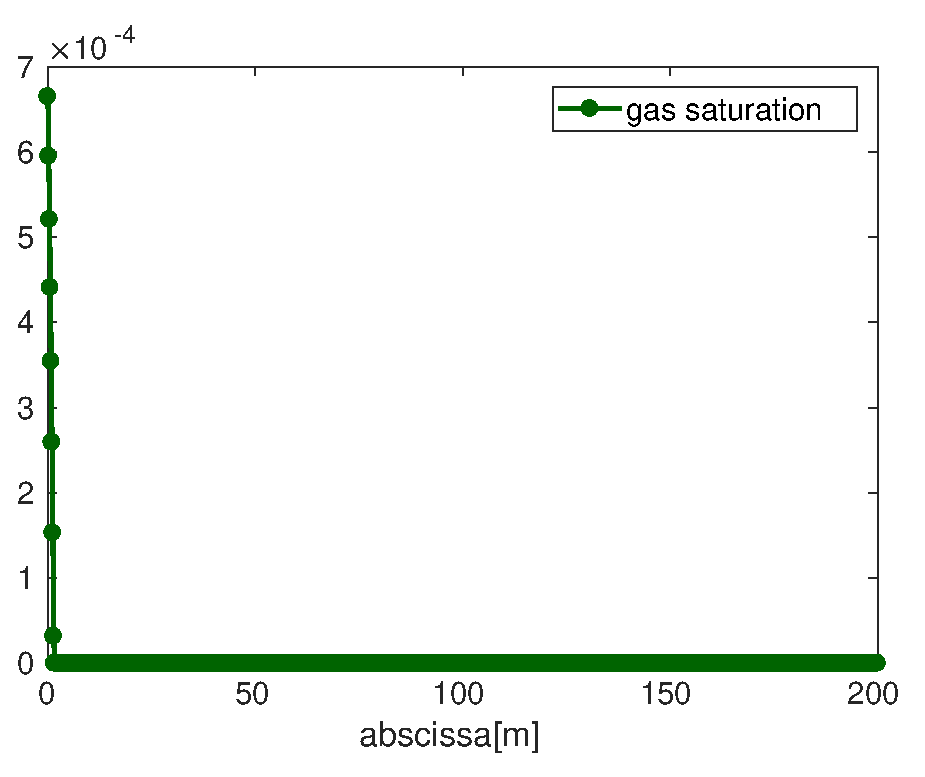
\includegraphics[width=0.45\textwidth]{fig_article_chap_3/satur_gas_appearance.eps}
 \quad
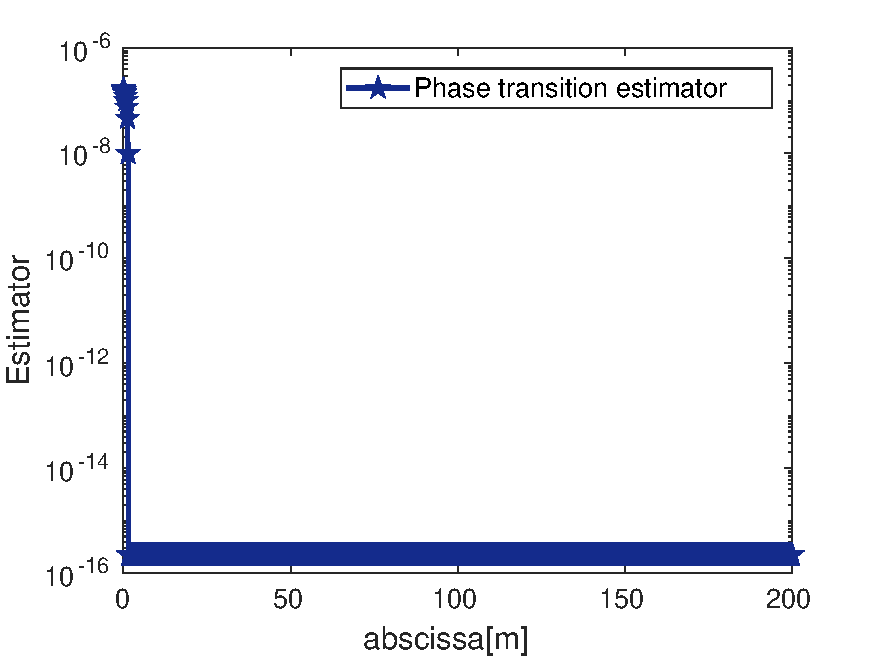
\includegraphics[width=0.47\textwidth]{fig_article_chap_3/MODIF_phase_transition_estimator_appearance_gas_nt=2_cv}
\end{figure}    

\onslide<3>
\scriptsize{ \textbf{\textcolor{red}{ \bm{$t = 4.25 \times 10^4$} years}}}
\begin{figure}
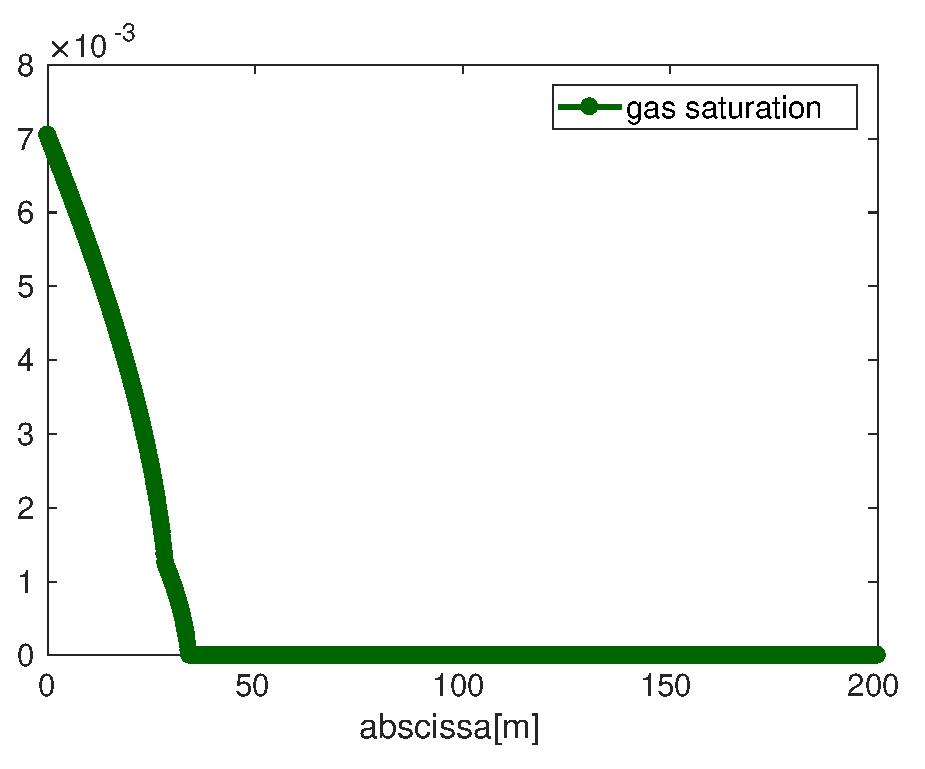
\includegraphics[width=0.45\textwidth]{fig_article_chap_3/satur_gas_after_appearance.eps}
\quad
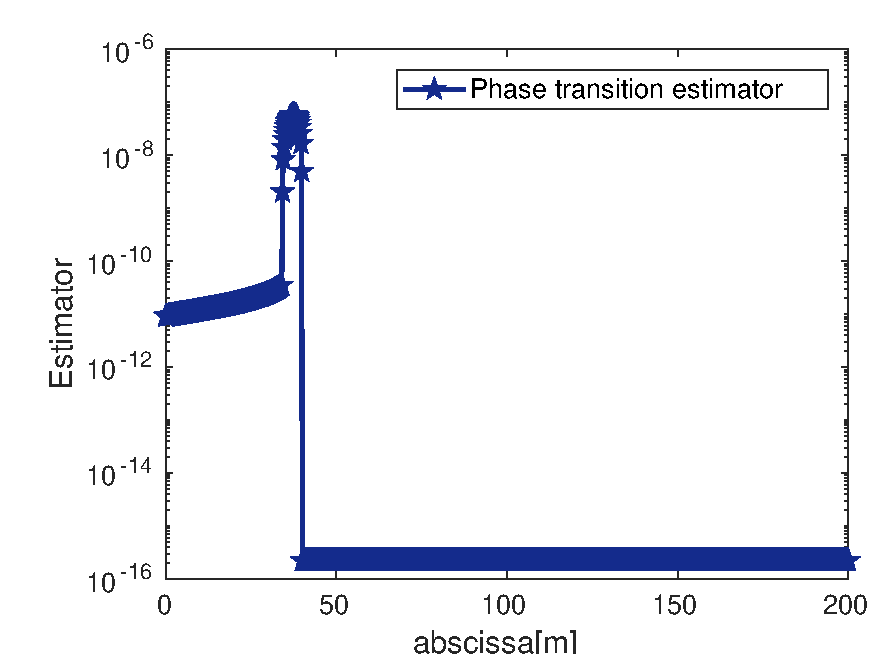
\includegraphics[width=0.47\textwidth]{fig_article_chap_3/MODIF_phase_transition_estimator_appearance_gas_nt=9_cv}
\end{figure}
\end{overprint}
 \end{frame}
%
\begin{frame}
\frametitle{Overall performance $\gammalin = \gammaalg = 10^{-3}$}
\begin{figure}
\centering
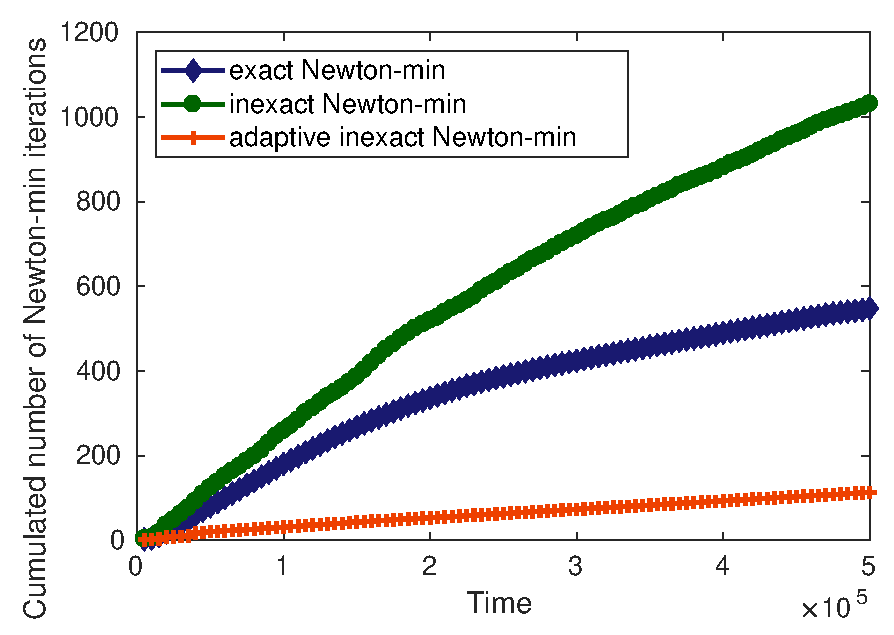
\includegraphics[width=0.47\textwidth]{fig_article_chap_3/Cumulated_number_Newton_iterations_three_methods_Nx_1000}
\hspace{0.6 cm}
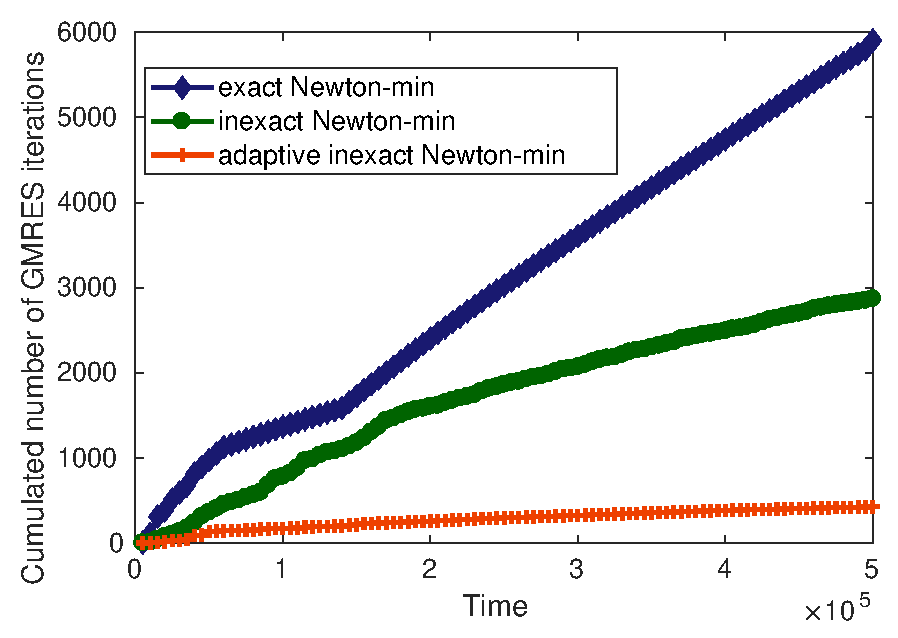
\includegraphics[width=0.47\textwidth]{fig_article_chap_3/Cumulated_number_gmres_iterations_three_methods_Nx_1000}
\end{figure}
\end{frame}
%
\begin{frame}
\frametitle{Accuracy $\gammalin = \gammaalg = 10^{-3}$}
\vspace{-0.1 cm}
\textcolor{cadmiumgreen}{\hspace{2 cm} $t = 1.05 \times 10^5$ years \hspace{5 cm} $t = 3.5 \times 10^5$ years}
\begin{figure}
\centering
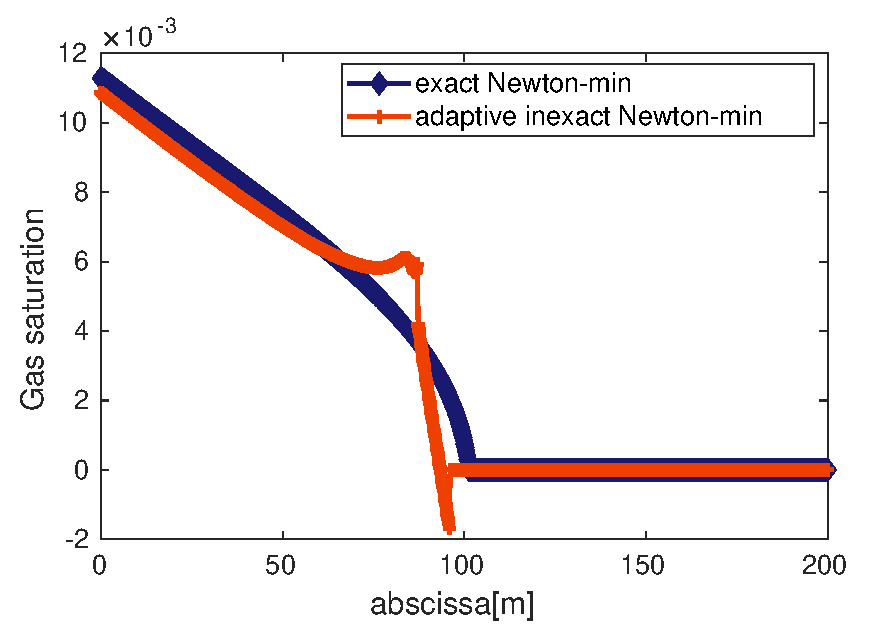
\includegraphics[width=0.48 \textwidth]{fig_article_chap_3/comparaison_plot_gas_saturations_exact_adapt_inexact_gamma_lin_gamma_alg_10-3_nt_21}
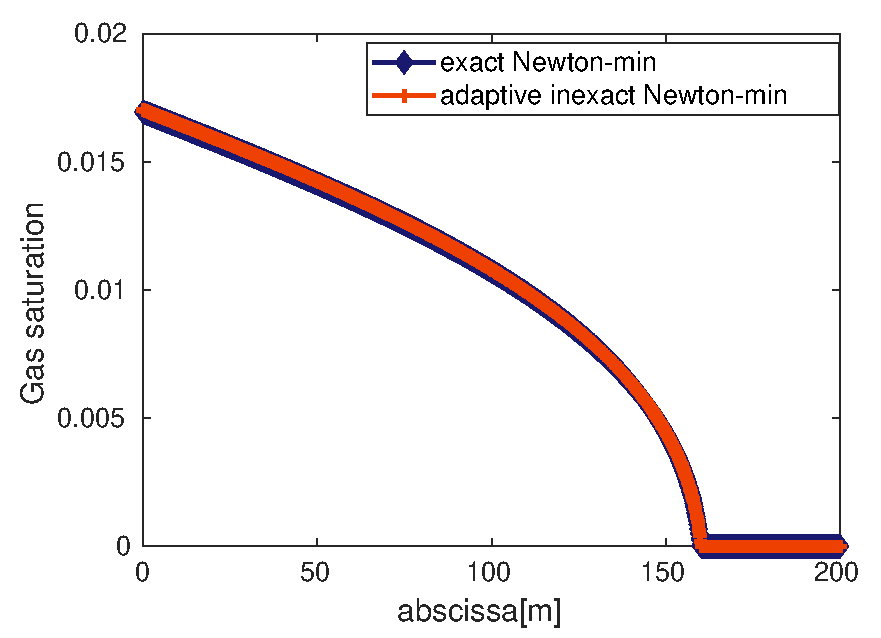
\includegraphics[width=0.48 \textwidth]{fig_article_chap_3/comparaison_plot_gas_saturations_exact_adapt_inexact_gamma_lin_gamma_alg_10-3_nt_70}
\end{figure}
\begin{thebibliography}{10}
 \scriptsize{
 \bibitem{Dabaghi:Martin:Vohralik:BenGharbia:2020}
 {\sc I.~Ben Gharbia J.~Dabaghi, V.~Martin, M.~Vohral\'{i}k}, A posteriori error estimates for a compositional two-phase flow
with nonlinear complementarity constraints.
\em{Computational Geosciences} (2020).
}
 \end{thebibliography}
\end{frame}
